% WP X: "WP name"
% Deliverable DX.Y: "Name of this deliverable"
%
% Editors: Name and Surname of the Editor
% List of Authors:
%

\documentclass{SmartReport}
\usepackage{url, rotating,todonotes, listings}
\let\svtodo\todo\renewcommand\todo[1]{\svtodo[inline]{#1}}
% \newcommand{\todo}[1]{\textcolor{blue}{#1}}

\usepackage{subfig}

\begin{document}
\wpnumber{8} \wptitle{Architecture and Integration}
\instshort{ShortNameInstitution} \delnumber{8.4} \versionnumber{0.1}
\contribshort{UH}
\deltitle{Final platform prototype and validation}
\delshorttitle{Platform Prototype} 
\delavail{PU}
\delstatus{D}	
\duedate{30/06/2016}
\deldate{\today}
\delowner{Daniele Miorandi, UH}
\wpleader{Iacopo Carreras, UH}
\qualityassessor{Luc Moreau, SOTON}
\smartkeywords{Platform, Prototype, Integration, Validation}
\maketitle

\newcommand{\mdl}{\textsc{SmartCOM}}

\begin{smartcontributors}
%%syntax: version number & date & author (institution) & reviewer (individual)\\
%0.1 & 04/11/2014 & 
UH & Tommaso Schiavinotto, Daniele Miorandi, Iacopo Carreras\\
UNITN & Ronald Chenu\\
SOTON & Heather Packer\\
BGU & Kobi Gal, Eran Yogev, Shaked Hindi\\
DFKI & Agnes Gruenerbl\\
UEDIN & Michael Rovatsos\\
\end{smartcontributors}

%define the abstract
\begin{smartabstract}
The SmartSociety platform represents a toolbox for easily and quickly building applications and services executing hybrid, diversity-aware forms of social computation. The toolbox includes eight components, each one performing a well-defined functionality and accessible through REST APIs. Functionality exposed by the components can be accessed by means of a set of programmer-friendly primitives, which are supported by a purposefully developed runtime library. 

The core components of the toolbox are released as open source form under a liberal licensing scheme, allowing researchers, Web entrepreneurs and startup companies to quickly prototype, deploy and experiment with applications and services enabling augmented collectives.

This report describes the final version of the SmartSociety platform, which integrates the instantiation of the components designed and developed by the Consortium members within the framework of the technical workpackages WP2-WP7. 




\end{smartabstract}


\section*{List of Acronyms}
\begin{tabular}{|c|p{3cm}|p{10cm}|}
\hline 
\textbf{Acronym} & \textbf{Full Name} & \textbf{Description} \\
\hline 
\hline 
%EC & Evaluator Component & System component in charge of evaluating the outcomes of each computation task (Sec.~\ref{sec:evaluator}).\\
%\hline 
CAS & Collective Adaptive System & Systems composed by heterogeneous entities that are autonomous but have to cooperate with each other to accomplish collective tasks.\\ \hline
HDA-CAS & Hybrid and Diversity-Aware Collective Adaptive System & A CAS where humans and machines `compose' by synergically complement each other thus bridging the semantic gap between low-level machine and high-level human interpretation of data and where they interoperate collectively to achieve their possibly conflicting goals both at individual and societal levels\\ \hline
API & Application Programming Interface & Set of tools and methods for accessing, from within a computer program, the functionality of an application/service \\ \hline
REST & Representational State Transfer & An architectural style of APIs, where the focus is on component roles and a specific set of interactions between data elements rather than implementation details.\\ \hline
CBT & Collective-Based Task & Object encapsulating all the necessary logic for managing complex collective-related operations \\ \hline 
CM & Context Manager & System component in charge of monitoring the
context the agent represented on the platform by a peer is in.\\
\hline
IM & Incentives Manager & System component in charge of managing the implementation of incentive schemes.\\  
\hline 
KB & Knowledge Base &  System component in charge of storing and managing the knowledge in the platform.\\
\hline
OM & Orchestration Manager &  System component in charge of
orchestrating the lifecycle of tasks on the SmartSociety platform. \\
\hline 
PF & Programming Framework &  System component in charge of exposing
appropriate primitives and interfaces to application developers.\\
\hline 
PM & Peer Manager &  System component in charge of managing peers.\\
\hline 
PS & Provenance Service & System component in charge of logging actions and information flows occurring on the platform.\\
\hline
RM & Reputation Manager & System component in charge of handling the reputation of any system resource, including peers. \\
\hline
SmartCom & Communication Middleware & System component in charge of managing
communication channels between the platform and the peers. \\
\hline
TEM & Task Execution Manager & System component in charge of
monitoring the execution of tasks and trigger corrective actions if
needed.\\
\hline
\end{tabular}

\newpage

%%%%%%%%%%%%%%%%%%%%%%%%%%%%%%%%%%%%%%%%%%%%%%%%%%%%%%%%%%%%%%%%%%%%%%%%%%%%%%%%%%%%%%%%%%%%%%%%%%%%%%%%%%%%%%%%%%%%%%%%
%%%%%%%%%%%%%%%%%%%%%%%%%%%%%%%%%%%%%%%%

\section{Introduction}
\label{sec:intro}
This report describes the final version of the SmartSociety platform. The corresponding software toolbox can be accessed at the following integrated repository:
\url{https://gitlab.com/smartsociety/}
% \footnote{A login/password has been created for reviewers: SmartSocietyReviewer/sm@rts0c13tyr3v13w3r}

% \todo{Put everything in a public repository (!) - check with partners}

The SmartSociety platform integrates the technical components, and provides the hooks to be able to operate a HDA-CAS. Generally speaking, a HDA-CAS is composed by peers (individuals, machines and collectives representing ensembles of the aforementioned) which coalesce around (and is enabled by) a service/application, which may run on top of the SmartSociety platform. The platform itself is therefore a technology enabler for the service/application which gives rise to the HDA-CAS. 

From the technical standpoint, the platform is shipped as a toolbox, and it includes eight components, each one performing a well-defined functionality and accessible through REST APIs. Functionality exposed by the components can be accessed directly or by means of a set of programmer-friendly primitives, supported by a purposefully developed runtime library. Java bindings are provided as part of the toolbox. 

The core components of the toolbox are released as open source form under a liberal licensing scheme (Apache v.2\footnote{http://www.apache.org/licenses/LICENSE-2.0}). This is in line with the mission of the SmartSociety, where the platform plays a pivotal role in allowing researchers, Web entrepreneurs and startup companies to quickly prototype, deploy and experiment with applications and services based upon hybrid and diversity-aware collectives.

% \todo{For reviewers only: add on enhancements since v. 2.0}
The final version of the platform builds upon v.2.0, which was delivered as D8.2~\cite{D8.2}. The enhancements include:
\begin{itemize}
\item Integration of the Task Execution Manager (TEM), the component in charge of monitoring the execution of tasks and identify deviations from the plan (and, in case, call the Orchestration Manager to provide a new plan);
\item Integration of the Incentive Server (IS), the component providing on-line recommendations on how to improve peer engagement;
\item Integration of the programming framework (PF), which provides primitives for programmers to easily access the platform functionalty.
\end{itemize}

% During the period M25-M30, the integration work continued along the roadmap included in D8.2~\cite{D8.2} leading to the integration of the provenance service, to the development and integration of the monitoring component, to the integration of the new version of the peer manager and to a refactoring of the runtime in order to align with the development of the programming model in WP7. Furthermore, some lab experiments were carried out to test and validate the platform functionalities and its ability to support the complete application life-cycle. 

The remainder of the deliverable is organized as follows. Sec.~\ref{sec:arch} describes the platform architecture and the overall functionality. Sec.~\ref{sec:sw} describes the platform components and their interfaces. Sec.~\ref{sec:val} describes how the platform can be used to build CASs and includes some basic examples. Sec.~\ref{sec:concl} concludes the report with an outlook on the future of the platform and its potential exploitation, together with some ethics considerations on the usage of the platform.

%Starting from the analysis of requirements and initial platform architecture in D8.1~\cite{D8.1}, WP8 undertook an intense dialogue with technical workpackages (WP2-WP7) in order to ensure full alignment of the top-level platform architecture and of the scientific and technical outcomes of WP2-WP7. The main result of this first phase was a revised architecture of the SmartSociety platform, which is presented in Sec.~\ref{sec:arch}. During the second half of the year the actual integration of components started, resulted in a 'minified' version of the platform, which integrates the Peer Manager (PM), the Orchestration Manager (OM) and the Communication Middleware (CM), plus an application runtime. For such aforementioned components, the interfaces used are summarised in Sec.~\ref{sec:apis}. The platform-level APIs and functionality are described in Sec.~\ref{sec:sw}. The missing components will be integrated during the third year according to the roadmap outlined in Sec.~\ref{sec:concl}.

% Within the SmartSociety project, Work-Package 8 (WP8) covers a twofold
% role. First, it is in charge of defining the architecture of
% the SmartSociety platform, ensuring a consistent view of the overall system, 
% as well of the components being developed by the various technical
% work-packages. Second, it aims at integrating the
% software components developed in the technical work-packages (WP2-WP7)
% into a coherent system prototype. Such prototype platform will be
% used to develop and validate the proof-of-concept applications realized in WP9.

% Within the first year of activities, only one task (T8.1, {\it Platform
% requirements analysis and design}) was active. Activities started, in
% line with the work plan, at M7. This deliverable
% includes therefore the outcomes of the activities undertaken by Consortium
% partners within the period M7-M12. 

% Activities focused on (i) the analysis of requirements for the SmartSociety platform (ii) its preliminary design in terms of system-level architecture. 

% High-level requirements were elicited by working in close cooperation with the
% other WPs. They are organized around the many heterogeneous dimensions involved in the design of a complex socio-technical system such as SmartSociety, and cover the properties
% that should be met by the final platform prototype. The analysis of the requirements represented the starting point for the design of the
% system-level architecture. \\
% The architectural design was inspired by four principles:
% \begin{itemize}
% \item {\bf Requirements:} the need to meet the requirements identified in the first part
% of the deliverable for the SmartSociety platform. Such requirements will affect the design of both the overall system, as well as of single modules and components.
% \item {\bf Integration:} the ability to provide a clear description of how the outcomes
% of the technical WPs (WP2-WP7) will be aligned and coherently integrated in the platform
% prototype.
% \item {\bf Flexibility:} supporting flexibility in the usage of the platform in order to
% enable the on-field experimental activities to be carried out for validation purposes in WP9. 
% \item {\bf 3E}: To promote the re-use of existing infrastructures, components and modules in the development process in order to meet the criteria of economy, efficiency and effectiveness. 
% \end{itemize}

% Based on these considerations, a first design of the overall platform architecture was carried out. It encompasses:
% \begin{itemize}
% \item the definition of the logical and functional role of each platform component. This includes also the preliminary identification of modules within each component, in line with the progress of single technical WPs (Logical View);
% \item the identification of how the various components interact with each other when running a computation (Dynamic View);
% \item a preliminary identification of the deployment constraints (Deployment View).
% \end{itemize}

% Finally, a sample mapping to one of the scenarios used in the first year by the Project Consortium, namely the ride sharing one, is reported. Ride sharing has been used by the Consortium as an illustrative example of a hybrid computation. This mapping is provided in order to help other WPs to achieve a better understanding of the functionalities and features to be provided by each component and of the interactions with other WPs.

% The architecture presented in this document will represent the starting point for the integration activities to be carried out in the second year of activities. The architecture will be iteratively revised, as the specifications of components by WP2-WP7 become available and scenarios and use cases get refined by WP9. The architecture of the SmartSociety platform should therefore be regarded as a reference living document, which will change and evolve over the life-time of the project. The adoption of an agile approach in the development and integration process will be adopted, with architectural design documentation getting updated at each release of the platform prototype. A first revised version of the architecture will be released together with the first prototype at M24 (D8.2). 

% The remainder of this deliverable is organized as follows. In
% Sec.~\ref{sec:requirements} we describe the requirements elicited for the
% SmartSociety platform. In Sec.~\ref{sec:design} we map such
% requirements to overall design patterns and principles, which
% constitute the basis for the architecture definition. The architecture
% is presented in terms of logical view in Sec.~\ref{sec:logical_view},
% of dynamic view in Sec.~\ref{sec:data_view} and of deployment view in
% Sec. \ref{sec:deployment_view}. A sample mapping to the ride-sharing scenario
% is provided in Sec.~\ref{sec:mapping_scenarios}.
% Sec.~\ref{sec:conclusions} concludes the deliverable defining a
% roadmap for the activities of WP8 in the second year of the project. 


%%%%%%%%%%%%%%%%%%%%%%%%%%%%%%%%%%%%%%%%
%%%%%%%%%%%%%%%%%%%%%%%%%%%%%%%%%%%%%%%%%%%%%%%%%%%%%%%%%%%%%%%%%%%%%%%%%%%%%%%%%%%%%%%%%%%%%%%%%%%%%%%%%%%%%%%%%%%%%%%%
\newpage


%%%%%%%%%%%%%%%%%%%%%%%%%%%%%%%%%%%%%%%%%%%%%%%%%%%%%%%%%%%%%%
\section{Platform Architecture}
\label{sec:arch}
% This section describes the final architecture of the SmartSociety platform. 
% In line with the iterative approach pursued by the Consortium, the description is a snapshot of the current status of project activities in terms of integration of technology and software modules developed, and will evolve during the remainder of project lifetime according to the roadmap described in Sec.~\ref{sec:concl}.
A high-level view of the SmartSociety platform architecture is presented in Fig.~\ref{fig:architecture}~\cite{scekic_soca2015}. 
%The architecture is designed to be fully distributed and scalable. 
The rectangle boxes represent the key platform components. All components expose RESTful APIs. The deployment can be centralized or distributed, depending on the specific use cases and constraints. 
%They can be deployed distributively, as all components expose (private or public) RESTful APIs. %The principal component-interoperability channels are denoted with double-headed arrows in the figure. 
%Communication with peers is additionally supported via popular commercial protocols to allow a broader integration with existing communication software and 

In general, we distinguish between the following relevant actors~\cite{D7.2}:
\begin{enumerate}
\item Users – external human clients or applications who require a task to be performed;
\item Peers – human or machine entities providing Human/Web Services to the platform;
\item Developers – external individuals providing the business logic in form of a programming language code that is compiled and executed on the platform in form of SmartSociety platform applications.
\end{enumerate}
In the SmartSociety framework peers typically perform tasks within collectives. A collective consists of a team of human and/or machine peers, whose formation and operations are purposefully supported by the platform.

% In order to ease inclusion of peers into the platform, interaction via popular commercial protocols and communication software (email, facebook, twitter, dropbox etc.) is also supported.

\begin{figure}[!ht]
 \centering
 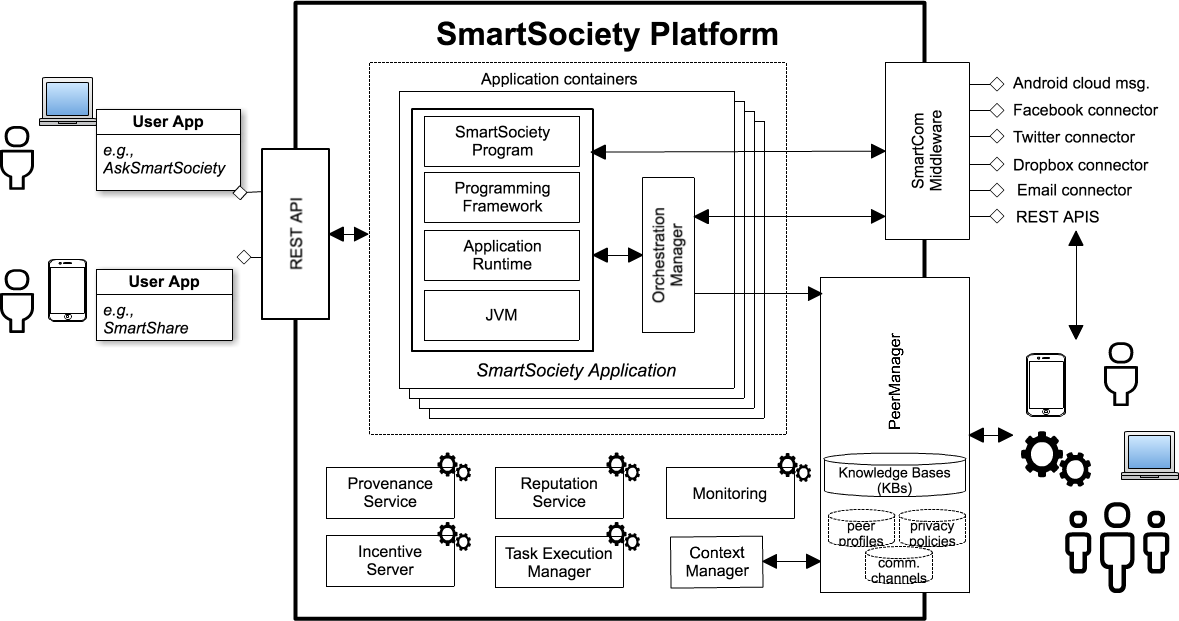
\includegraphics[width=\linewidth]{figs/architecture_v3}%platform-architecture}
 \caption{SmartSociety platform users and architecture.}
 \label{fig:architecture}
\end{figure}

% User applications contact the platform through the REST API component.
% All incoming user requests are served by this module that %verifies their correctness and 
% dispatches them to the appropriate platform application, which will be processing and responding to them. 
% The platform applications run sandboxed in Docker \footnote{\url{https://www.docker.com/}} containers. The applications can be deployed on different (virtual) machines.
% %
% %
% Applications request from the Peer Manager a set of permissions for accessing and manipulating personal private data of peers. The Peer Manager can shortly be described as the central information system of the platform, managing all peer and application information, and allowing privacy-aware access and sharing of the data among platform components. 
% %
% The platform application %is a Java application 
% makes use of SmartSociety platform's programming libraries, allowing the developer to execute collective-based tasks on the platform. 
% %
% Each platform application features a dedicated \emph{Orchestration Manager (OM)} component. The OM is the component in charge of preparing and orchestrating collaborative activities among peers. Performing these functionalities requires the OM to heavily use the Peer Manager and \mdl{} Middleware components. 


From the logical standpoint, the platform includes eight components, each one performing a well-defined functionality and accessible through REST APIs. Functionality exposed by the components can be accessed by means of a set of programmer-friendly primitives (through the so-called Programming Framework), which are supported by a purposefully developed runtime library. Java bindings are provided as part of the toolbox. 
The platform components are:
% For the sake of Below we briefly report a description of each component.

% During the second year of project activities integration activities
% started. In the integration process, the architecture initially
% presented in Deliverable D8.1 was deeply revised. This process was
% required in order to align the activities carried out within the
% project's technical work packages (WP2-WP7) and to ensure
% interoperability among the components developed by the various
% partners. In this section we briefly present the architecture as it
% currently stands (at M24). No major changes are currently foreseen,
% even if ---given the research-oriented nature of the SmartSociety
% project--- this cannot be guaranteed. In this sense, the architectural
% specifications of the SmartSociety platform have to be seen as a live document, which reflects the
% actual progress of the research activities carried out by Consortium
% partners. 

%\subsection{Logical View}
%The logical view of the SmartSociety platform is presented in Fig.~\ref{fig:logical_view}. %The Consortium has identified 9 key
%components which jointly provide the required system-level functionality.

%\begin{sidewaysfigure}
%\begin{figure}[!hbt]
% \centering
% \includegraphics[width=1\textwidth]{figs/functional_diagram}%logical_view.pdf}
% \caption{SmartSociety logical view.}
% \label{fig:logical_view}
%\end{figure}
%\end{sidewaysfigure}

%\todo{Update ref to figure (take from collaboratecom paper) + shorten description of components}
% A brief description of the functionality of the components integrated is reported here for the sake of completeness.
%The core components which are part of the revised version of the SmartSociety are the following:
\begin{itemize}
% \todo{questa c'e' ancora?}
% \item \textbf{Application Runtime}: this is the component providing the support logic enabling peers to execute tasks. The runtime provides handlers for interacting with the various internal components provided by the SmartSociety platform~\cite{D8.3}. The Application Runtime provides the main endpoint for external applications to interact with the SmartSociety platform. \todo{questa c'e' ancora?}%The Application Runtime is developed within WP8. 

\item \textbf{Orchestration Manager (OM)}: it provides two key functionalities: composition and negotiation~\cite{D6.2}. Composition takes task requests as inputs and generates tasks by solving constraint satisfaction problems specific to each application, potentially interacting with the peer manager (so that peer with certain capabilities can be identified) and the reputation service (so that the reputation of the capable peers can be obtained). The composition determines (i) the peers which can potentially execute such task, and (ii) the necessary interactions and/or external services which are needed to execute such task.  The negotiation manager is in charge of handling the negotiation process with peers in order to ensure that the services and resources required to carry out the task are actually present. %The Orchestration Manager (OM) is developed within WP6 and its description can be found in~\cite{D6.2}.

\item \textbf{Peer Manager (PM)}: it is responsible for managing peer-related information~\cite{D4.3}. This includes their profile, as well as any other information which will be used by the Orchestration Manager for identifying possible peers that can execute a given task.  It maintains a profile of each peer, which
represents a model thereof in terms of knowledge, resources and
capacity. It provides a peer search functionality that is used by the Orchestration Manager to create compositions. Besides individual peers, the Peer Manager also manages collectives, which are groups of peers characterized by specific properties. %Besides managing peer-related information, 
The Peer Manager includes a set of mechanisms for ensuring the user's privacy~\cite{D4.3}.
%s also in charge of protecting the user's privacy. 
%The Peer Manager embeds a Knowledge Base (KB), which contains an agreed ontology about peers, task, workflows, incentives, etc. The KB provides the domain terminology, as well as all the semantic relations between terms. The KB is responsible for ensuring that all component share a common understanding of the inputs/outputs between any two parties of the platform. The overall KM is divided into domains, which allow to capture the diversity of the entities being part of SmartSociety. A semantic reasoner will allow to perform semantic queries over the KB. %The Peer Manager (PM) is developed within WP4 and its description can be found in~\cite{D4.3} .

\item \textbf{Task Execution Manager (TEM):} %\todo{Add description, take from slides resulting from the Frankfurt meeting with WP3/WP6} 
The TEM is in charge of managing the task execution phase. In particular it monitors whether the task execution is in line with expected plan (taken from the task description). In case a deviation is detected, it might trigger a re-planning by using OM's functionality. 
%takes as input a description of the task under execution and data about the actual status of peers (mediated by the PM) to understand the level of completion and to trigger, if needed, appropriate actions by the OM.

\item \textbf{Context Manager (CM):} it is responsible for monitoring the context the agent represented on the platform by a peer is in~\cite{D3.2}. For an individual human agent, this includes, e.g., tracking the location and recognizing the activity the agent is currently involved in. This can be further used to trigger context adaptation in applications. The %The Context Manager (CM) is developed within WP3 and a high-level description can be found in~\cite{D3.2}.

\item \textbf{Reputation Service (RS):} it handles the reputation of any system resource, including peers ~\cite{D2.3}. It computes the reputation of a given peer based on feedback from other peers. % and users. %It uses data from the provenance store in order to carry out the computation. Reputation is based on various metrics that the system will be able to compute, starting from peers' execution of tasks. 
Reputation information can be exposed directly to application users or used by the PM in the selection of suitable peers for a given task. %The Reputation Manager (RM) is developed within WP2. A description of the RM can be found in ~\cite{D2.3}.

%\item \textbf{Knowledge Base}: it is shared among the various components of the platform, and contains an agreed ontology about peers, task, workflows, incentives, etc. It provides the domain terminology, as well as all the semantic relations between terms. In particular, the knowledge base is responsible for ensuring that all component share a common understanding of the inputs/outputs between any two parties of the platform. The overall knowledge base will be divided into domains, which allow to capture the diversity of the entities being part of SmartSociety. A semantic reasoner will allow to perform semantic queries over the knowledge base.

\item \textbf{Provenance Service (PROV):} it logs descriptions of actions performed by platform
components and peers, as well as information flows between them, according to the W3C PROV recommendation~\cite{D2.2}. In particular, it includes the provenance store, a component responsible for keeping a record of how the overall compositions are being created, executed and how the data managed by the platform is being transformed. %It will play a fundamental role in the evaluation of peers reputation. %, as well as in ensuring that the system as a whole enforces the proper privacy constraints imposed by the peers.
%It further supports an explanation service, which is able to visualize provenance trails and convert them in natural language. The Provenance Store (PS) is developed within WP2. A description of the PS can be found in~\cite{D2.2}.

\item {\bf Monitoring and analysis service (MONITOR):} it logs and monitors the platform jobs and can be used by platform administrators to check the liveness of the platform services, to perform root-cause analysis and to extract analytics on the performance of the system~\cite{D8.3}. 

\item {\bf Incentives server (IS):} it manages incentives and
interventions that can be used to achieve higher quality results. Incentives %can play a twofold role in SmartSociety. First, they 
can be used to stimulate the participation of a peer (or a collective) in the execution of a given task 
%. Second, they 
or can be used to define specific strategies for community engagement~\cite{D5.4}. %This will play a fundamental role in maintaining the peers community active over time. The Incentives Manager (IM) is developed within WP5.
\end{itemize} 	


% \subsection{Deployment View and Network Diagrams}
% The SmartSociety platform has been designed according to REST architectural principles, with the aim of supporting flexibility in the deployment model. %This means that 
% The platform seamlessly supports both single-tenant as
% well as multi-tenant deployment models. %Also, 
% The platform components
% can be centralised on a single infrastructure or can be distributed
% across different servers. \todo{update diagram}
% %The choice of the specific deployment model
% %to be used depends on technical as well as business considerations. In
% %the remainder of this section we present, as a use case, the current
% %deployment utilised for integration, testing, validation and
% %experimentation purposes. This is by no means to be considered the
% %only model supported, but it provides an illustrative example of a
% %supported configuration. 

% \begin{figure}[!hbt]
%  \centering
%  \includegraphics[width=1\textwidth]{figs/netDiagram}
%  \caption{SmartSociety platform: network diagram}
%  \label{fig:netDiagram}
% \end{figure}

% A sample network diagram is reported in Fig.~\ref{fig:netDiagram}. The end user in this case interacts with a User Application running on her smartphone. The mobile app interacts with the Application residing in the SmartSociety Platform Core Deployment. %Some of the components reside on different servers; 
% In this sample case the PM is hosted by partner DISI and the PS and RM are hosted by partner SOTON. The Core Deployment further manages interactions with peers (through the CM). In this case we have a human agent which interacts through a Peer Mobile Application, a machine peer (Google) and a machine peer (Twitter) which then reaches out to human agents interacting with it through any Twitter client.



% The corresponding deployment diagram is reported in Fig.~\ref{fig:deployDiagram}. Here it can be seen that the core deployment server hosts four key components, i.e., the incentives manager, the communication middleware, the orchestration manager and the application container (where the application is executed). On the end user smartphone, besides the user application (client), the client of the context manager is also  deployed. The CM client interacts with the corresponding server-side component deployed on the DISI server, where the PM is also hosted. The PS and RM are on the SOTON server. A third-party server is used to host both Google and Twitter peer, which then connect to the corresponding web service. \todo{update diagram}
% \begin{sidewaysfigure}
% %\begin{figure}[!hbt]
%  \centering
%  \includegraphics[width=1\textwidth]{figs/deploymentView}
%  \caption{SmartSociety platform: deployment diagram}
%  \label{fig:deployDiagram}
% %\end{figure}
% \end{sidewaysfigure}

% \subsection{Dynamic View}
% Fig.~\ref{fig:dynamic_view} provides a sample dynamic view of how the various components of the SmartSociety platform interact with each other, when running an application based on SmartSociety.\footnote{For the sake of clarity, and as these were developed while integrating the first version of the platform, only interactions among the user application, application, orchestration manager, peer manager, communication middleware and human agents are reported.} \todo{update diagram}
% \begin{sidewaysfigure}
% %\begin{figure}[!hbt]
%  \centering
%  \includegraphics[width=1\textwidth]{figs/dynamic_view}
%  \caption{SmartSociety dynamic view .}
%  \label{fig:dynamic_view}
% %\end{figure}
% \end{sidewaysfigure}

% The sequence diagram can be summarized by the following steps:
% \begin{itemize}
% \item Platform invocation (step 1): the starting point is a user application (e.g., a mobile application) which is exploiting the SmartSociety platform for running a human computation task (refer to Sec.~\ref{sec:asksmartsoc} for a more concrete example). The request is directed towards an application deployed in the SmartSociety application container and providing the necessary support for executing the requested task. The invocation will contain all the necessary metadata, including a complete description of the task, according to the APIs offered by the application running in the platform.

% \item Composition request (steps 2-6): the application, after receiving the request from the user application, converts it into a \textit{composition job request}. A composition is the request to create a composition of peers/collectives capable of executing the task. The composition job request happens through %the programming abstractions provided by 
% the runtime, which allows to fully characterize the task that needs to be executed. Creating a composition involves querying the Peer Manager for identifying peers capable (individually or all together) to perform the given task\footnote{Note that also the Reputation Manager can be queried during this process. This is not reported in the diagram for the sake of simplicity, and as it reflects the current integrated components.}. Once the composition is identified, it is returned to the application, together with a pointer to the peers involved in it.

% \item  Negotiation (steps 7-14): the application then negotiates with peers the participation of the agents they represent in a given task. This is mediated/facilitated by the Orchestration Manager. Such negotiation occurs for every single peer involved in the identified composition. The negotiation with peers also involves the identification of the channel preferred by the peer to receive a given task (e.g., email, social, mobile app in the case of human agent). In this phase, the SmartCom communication middleware is exploited to facilitate the interaction with peers. At the completion of this phase, the Orchestration Manager is notified about the successful completion of the negotiation.

% \item Execution (steps 15-20): once the composition has been successfully identified and agreed with peers, the execution of the task can starts. This can be based over multiple steps and is managed by the Application, exploiting the programming framework provided be the application runtime. This phase concludes with the complete execution of the submitted task. Results are then returned to the User application that has initiated the request.

% \end{itemize}


% % The SmartSociety platform is meant to support a rather wide range of
% % social computation patterns (or templates). In order to provide
% % insight into the flexibility of the platform and the actual
% % interworking of components, we have developed sequence diagrams for two
% % 'extreme' applications:
% % \begin{itemize}
% % \item SmartShare is a ridesharing system able to account for user's
% % preferences and to compute recommendations based on the feedback
% % provided by other service users. It is what we call a 'full
% % negotiation' scenario, in which the computational task of finding an
% % agreement on the rides is left to individuals and collectives. The
% % platform in this case is used to carry out administration tasks, in
% % particular keeping track of the rides and ride requests, their status
% % and to maintain reputation of drivers and passengers.
% % \item AskSmartSociety! is a Q\&A service supporting hybridity. The
% % computational pattern here is that typical of micro-tasking
% % applications (\'a la Mechanical Turk, roughly speaking), where the
% % task in this corresponds to a question to be answered. The service
% % supports hybrid computation in that questions can be transparently
% % provided by machine peers or human peers. Quality criteria can be
% % specified in order to define when a chosen answer has to be presented
% % to the user. 
% % \end{itemize}
% % In the following we present details about the two aforementioned
% % applications. 
% % \subsubsection{Example: SmartShare}
% % \begin{figure}
% % \centering
% % \includegraphics[width=0.9\textwidth]{./figs/sequenceRide}
% % \caption{Sequence diagram of the SmartShare application.}
% % \label{fig:dynamic_share}
% % \end{figure}

% % \subsection{Example: Ask SmartSociety}\label{sec:asksmartsoc}
% % \textit{Ask SmartSociety} is a simple Questions and Answer service enabled by the SmartSociety platform which has been used as the benchamark for implementing the initial version of the SmartSociety platform. It focus on tourism, which is the reference domain to be used for validating the SmartSociety vision.\\
% % Ask SmartSociety! will be a service where users can post questions in natural languages and peers can provide answers. Peers providing answers can be humans (individuals or collectives) as well as machines (intelligent software agents). Peers can compose (forming collectives, hybrid or not) to provide answers. Answers can be ranked based on the reputation of the peers or on community ranking (similarly to stackoverflow). In some instances the user issuing the question can select an answer and provide feedback on the peer providing it.
% % Two examples (grounded in the tourism application scenarios) can help in understanding the features of the Ask SmartSociety! service:

% % \textit{Next week Peter will fly to Venice. He will be busy in meetings during the day but wants to explore some ‘hidden’ places at night. He could well explore various online tourist sites but he prefers to ask experts and local people. He could also google for relevant content, but he does not actually need an answer right away, he just needs to get it in one week. And having one system which allows him to query local experts, web-based recommendation services and incoming tourism institutions looks definitely appealing to him!
% % Alice is visiting Milano during the next week. It is his first time in Milan, and she is looking for a restaurant in the city centre. Since it is spring time, she would love eat outside and therefore  find a restaurant with a garden. Alice is also celiac, and she needs to find restaurants, which do have gluten free menus. She relies on the Ask SmartSociety! application for retrieving some suggestions on where to have dinner during her stay in Milan. She is looking for unconventional recommendations.}


% % \begin{figure}
% % \centering
% % \includegraphics[width=0.9\textwidth]{./figs/sequenceAsk}
% % \caption{Sequence diagram for AskSmartSociety! applications.}
% % \label{fig:dynamic_ask}
% % \end{figure}
%%%%%%%%%%%%%%%%%%%%%%%%%%%%%%%%%%%%%%%%%%%%%%%%%%%%%%%%%%%%%%
\newpage

% %%%%%%%%%%%%%%%%%%%%%%%%%%%%%%%%%%%%%%%%%%%%%%%%%%%%%%%%%%%%%%
% \section{Mapping to the Application Scenarios}
% \label{sec:mapping}
% \input{sections/apps.tex}
% %%%%%%%%%%%%%%%%%%%%%%%%%%%%%%%%%%%%%%%%%%%%%%%%%%%%%%%%%%%%%%
% \newpage

% %%%%%%%%%%%%%%%%%%%%%%%%%%%%%%%%%%%%%%%%%%%%%%%%%%%%%%%%%%%%%%
% \section{Interfaces Specifications}
% \label{sec:apis}
% \input{sections/interfaces.tex}
% %%%%%%%%%%%%%%%%%%%%%%%%%%%%%%%%%%%%%%%%%%%%%%%%%%%%%%%%%%%%%%
% \newpage


%%%%%%%%%%%%%%%%%%%%%%%%%%%%%%%%%%%%%%%%%%%%%%%%%%%%%%%%%%%%%%
\section{SmartSociety Platform Components and Their APIs}
\label{sec:sw}
%!TEX root = ../main.tex
In this section we describe the software artifacts being produced, together with a description of their APIs.

\subsection{Orchestration Manager}
\subsubsection{Functionality and Features}
The OM provides collective composition and negotiation functionality. They can be invoked subsequently or jointly (in the latter case we talk about continuous orchestration, see~\cite{D6.2} for a detailed description. The OM takes as input task requests and outputs an agreed execution plan. 
\subsubsection{Implementation}
The OM implementation shipped with the toolbox is written in Javascript and based upon the node.js framework. It uses express for REST APIs, jade as node template and includes a mongoDB instance for persistency. Two versions are provided, supporting AskSmartSociety! and SmartShare applications. They can be easily reused to develop application-specific OMs.
\subsubsection{Interfaces, Endpoints and Resources Exposed}
\todo{taken from D2.3 - appendix}
For convenience we split the API into different sections.
B.1.1 Task Requests
We start with task requests. The most basic operations are listed in the following table:
 
verb
URI
POST
/applications/:app/taskRequests
GET
/applications/:app/taskRequests/?user=:user
GET
/applications/:app/taskRequests/:taskRequestID
HEAD
/applications/:app/taskRequests/:taskRequestID
GET
/applications/:app/taskRequests/:taskRequestID/v/:version
DELETE
/applications/:app/taskRequests/:taskRequestID
Create Task Request: POST /applications/:app/taskRequests This is the main URI where new task requests are posted. The JSON object describing the task request is expected in the body of the request. On success a platform call to the composition manager will be made.
Access Control. Any peer or user.
Success. Returns error code 201 together with
• a JSON document of the form {
28 of 57
http://www.smart-society-project.eu
Deliverable D2.3 ⃝c SmartSociety Consortium 2013-2017 data: aURI
}
where aURI is the URI where the client can retrieve (assuming authentication and access control policies have no issues) the latest version of the task request that has been posted, and optionally
• an ETag for the JSON object of the response.


Get Task Requests of User:
GET /applications/:app/taskRequests/?user=:user apart from authentication purposes (in the header).
Access Control. The peer user or an admin. Success. Returns error code 200 together with
• a JSON document of the form {
No parameters are expected
      data: [[userTaskRequestsURIs], [associatedETags]]
    }

    Get a Task Request:
GET /applications/:app/taskRequests/:taskRequestID No parameters are ex- pected apart from authentication information (if needed).
Access Control. The owner of the task request or an admin.
Success. Returns error code 200 together with the JSON document of the latest
version of the task request accompanied by the ETag of the document.
Failure. Returns an error code (403, 404) together with an optional error message.
Get the Head of a Task Request:
HEAD /applications/:app/taskRequests/:taskRequestID Similar to
GET /applications/:app/taskRequests/:taskRequestIDexceptthatthebodyreturned is empty. It just returns the ETag of the latest version of the task request to indicate if there has been a change to the document and thus we need to retrieve its latest version. The access control policy is similar as above; the owner of the task request or an admin can perform the operation.
Get a Specific Version of a Task Request:
GET /applications/:app/taskRequests/:taskRequestID/v/:version No param- eters are expected apart from authentication purposes (if needed).
Access Control. The owner of the task request or an admin.
Success. Returns error code 200 together with the specific version of the task request. Failure. Returns an error code together with an optional error message.
Delete a Task Request: DELETE /applications/:app/taskRequests/:taskRequestID
This is the main URI for deleting task requests. No parameters are expected apart from authentication information (in the header). A platform job is prepared and is posted to the deletion manager.
Access Control. The owner of the task request or an admin.

B.1.2 Tasks
Tasks are generated through composition (more on that below). The most basic operations related to them are listed in the following table:
 
verb
URI
GET
/applications/:app/tasks/:taskID
HEAD
/applications/:app/tasks/:taskID
GET
/applications/:app/tasks/:taskID/v/:version
PUT
/applications/:app/tasks/:taskID
Get a Specific Task: GET /applications/:app/tasks/:taskID Similar to GET /applications/:app/taskRequests/:taskRequestID but referring to tasks. No param- eters are expected apart from authentication information (if needed).
Access Control. The participants of the task or an admin.
Success. Returns error code 200 together with the JSON document of the latest
version of the task accompanied by the ETag of the document.
Failure. Returns an error code (403, 404) together with an optional error message.
Get the Head of a Task: HEAD /applications/:app/tasks/:taskID Similar as above but the body of the response is empty. Essentially this is an easy way for the clients to figure out if the resource has changed. Same access control policy as above.
Get a Specific Version of a Task:
GET /applications/:app/tasks/:taskID/v/:version No parameters are expected apart from authentication information (if needed).
Access Control. The participants of the task or an admin.
⃝c SmartSociety Consortium 2013-2017 31 of 57
⃝c SmartSociety Consortium 2013-2017 Deliverable D2.3 Success. Returns error code 200 together with the specific version of the task.
Failure. Returns an error code together with an optional error message.
Negotiate on a Task: PUT /applications/:app/tasks/:taskID The main call for negotiation which will trigger an additional platform call to the negotiation manager. Expects the new version of the document of the task taskID. A platform job for negotiation is prepared and is posted to the negotiation manager.
Access Control. The participants of the task or an admin.
Success. Returns error code 200 together with the new version of the task as is
dictated by the negotiation manager.
Failure. Returns an error code together with an optional error message.
B.1.3 Task Records
Task records are generated by the orchestrator once execution can start on a specific task. The most basic operations are listed in the following table:
 
verb
URI
GET
/applications/:app/taskRecords/:taskRecordID
HEAD
/applications/:app/taskRecords/:taskRecordID
GET
/applications/:app/taskRecords/:taskRecordID/v/:version
PUT
/applications/:app/taskRecords/:taskRecordID

Get a Specific Task Record:
GET /applications/:app/taskRecords/:taskRecordID No parameters are expected apart from authentication information (if needed).
Access Control. The participants of the task or an admin.
Success. Returns error code 200 together with the json document of the latest version
of the task record accompanied by the ETag of the document.

Get the Head of a Task Record:
HEAD /applications/:app/taskRecords/:taskRecordID No parameters are ex- pected apart from authentication information (if needed).
The body of the response is empty. This is another convenience function which allows an easy way for the clients to figure out if the resource has changed. Same access control policy and error codes as above.
Get a Specific Version of a Task Record:
GET /applications/:app/taskRecords/:taskRecordID/v/:version No parameters are expected apart from authentication purposes (if needed).
Access Control. The participants of the task or an admin.
Success. Returns error code 200 together with the specific version of the task. Failure. Returns an error code together with an optional error message.
Provide Execution Feedback:
PUT /applications/:app/taskRecords/:taskRecordID The main call for execu- tion which will trigger an additional platform call to the execution manager. Expects the new version of the task record document taskRecordID. A platform job for execution is prepared and is posted to the execution manager.
Access Control. The participants of the task or an admin.
Success. Returns error code 200 together with the new version of the task as dictated
by the execution manager.
Failure. Returns an error code together with an optional error message.

B.2 Composition Manager
The composition manager provides the following functionality:
verb
URI
POST
/applications/:app/compositions
GET
/applications/:app/compositions/:compositionID

Perform Composition: POST /applications/:app/compositions Expects the plat- form job with the description, for which the main ingredient is the new task request that has arrived on the platform.
Access Control. The orchestrator for the application app can make such a call.
Returns. The call always succeeds and generates a resource describing the outcome of composition. Upon completion it returns an error code 201 and the link to the document with the results of composition. Part of the description of the document with the results of the composition is the error code and message that is returned through the call POST /applications/:app/taskRequests to the client.
Get Composition Results:
GET /applications/:app/compositions/:compositionID No parameters are ex- pected.
Access Control. The orchestrator for the application app or an admin can make such a call.
Success. Returns error code 200, the JSON document with the description of the results of the composition together with the associated ETag for the document.
Failure. Returns an error code (e.g. 404 not found) together with an optional error message.
Comment. Normally such a call is expected to happen only once from the applica- tion orchestrator once the latter has received the 201 error code that the composition that was requested has been performed.

B.3 Negotiation Manager
The negotiation manager provides the following functionality.
Perform Negotiation: POST /applications/:app/negotiations Expects the plat- form job with the description, for which the main ingredient is the task on which negoti- ation is being performed.
Access Control. The orchestrator for the application app can make such a call.
Returns. The call always succeeds and generates a resource describing the outcome of negotiation. Upon completion it returns an error code 201 and the link to the document with the results of the negotiation. Part of the description of the document with the results of the negotiation is the error code and message that is returned through the call PUT /applications/:app/tasks/:taskID to the client.
Get Negotiation Results:
GET /applications/:app/negotiations/:negotiationID No parameters are expected.
Access Control. The orchestrator for the application app or an admin can make such a call.
Success. Returns error code 200, the JSON document with the description of the results of the negotiation together with the associated ETag for the document.
Failure. Returns an error code (e.g. 404 not found) together with an optional error message.
Comment. Normally such a call is expected to happen only once from the applica- tion orchestrator once the latter has received the 201 error code that the negotiation that was requested has been performed.
⃝c SmartSociety Consortium 2013-2017 35 of 57
 
verb
URI
POST
/applications/:app/negotiations
GET
/applications/:app/negotiations/:negotiationID



\subsubsection{Repository}
The OM code is available (Apache v.2) at: \url{https://gitlab.com/smartsociety/orchestration}

\subsection{Peer Manager}
\subsubsection{Functionality and Features}
The Peer Manager (PM) provides a peer-centered data store that maintains and manages information about human- or machine-based peers within a privacy-preserving framework.
The PM was designed with the objective of keeping the information owned by peers private. In order to provide a flexible management of information, the PM builds upon the notion of an entity-centric semantic enhanced model that defines an extensible set of entity schemas providing the templates for an attribute-based representation of peers’ characteristics~\cite{D4.2}. Additionally, the PM defines a storage and privacy protection model by adding privacy regulations and considerations. The PM is designed to comply with the recent General Data Protection Regulation (GDPR) (Regulation (EU) 2016/679).
\subsubsection{Implementation}
Not applicable, the PM is owned by University of Trento and implementation details are not made public.
\subsubsection{Interfaces, Endpoints and Resources Exposed}
% \todo{add from https://docs.google.com/spreadsheets/d/1UlRKshoALlSzmJYZVLkuzAGTUukdFKaONlKqPmd3RWo/edit#gid=0}
% \todo{@Ronald: please check the APIs \& also whether we can share them (deliverable is PU)}
We divide APIs in chapters. Let us start with the security ones:
\begin{itemize}
\item {\bf POST /security/login} Used for authentication. The call includes as parameters an identifier and a password, and returns, among the other data, a token to be used for further interactions with the platform.
\item {\bf POST /security/logout} Log the peer out of the PM.
\item {\bf GET /person} Read the person of a given logged user. 
\item {\bf GET /person\_sl?username=:username\&password=:password} Register a new human peer. Returns a peer ID. 
\end{itemize}
The second set of APIs cover management operations:
\begin{itemize}
\item {\bf GET /search}. General search machinery. Check~\cite{D4.3} for more explanations on the query language to be used. 	
\item {\bf POST /collectives} Create collective: create a collective structure from a set of usernames.
\item {\bf GET /collectives/identifier}	Return the usernames of all peers in a collective.				
\item {\bf DELETE /collectives/} Delete the collective with a given id.	
\item {\bf GET /types} Return the names and id of all the types defined in the peer manager.
\item {\bf GET /types/:id} Return a list of all the attributes for the given type id.
\item {\bf POST /instances} Create a new instance from a given type and its attributes values. 
\item {\bf GET /instances/:id} Return the type and the attribute values for the given instance.
\item {\bf PUT /instances/:id} Update one or more attributes for a given instance id (only attributes passed as in this call will be affected).											
\item {\bf DELETE /instances/:id } Delete the instance structure with the given id.						
\item {\bf POST /profiles} Create a new profile from an existing instance, a transformation and a policy.
\item {\bf GET /profiles/:id} Read profile by id: returns the type, the transformation, the policy and the attribute values for the given profile. 
\item {\bf DELETE /profiles/:id} Delete profile by id: delete the profile structure with the given id.	
\item {\bf POST /transformations}  Create a new transformation specifying the source type, the destination type and the attribute transformations to be performed.
\item {\bf GET /transformations/:id} Read transformation by id: return the source type, the destination type, and the attribute transformations for the given transformation.									
\item {\bf DELETE /transformations/:id} Delete transformation by id: delete the transformation structure with the given id.	
\item {\bf POST /policies} Create a new policy by specifying its use concept and validity limit.		
\item {\bf GET /policies/:id} Read policy by id: return the use concept and validity limit for the given policy.
\item {\bf DELETE /policies/:id} Delete policy by id: delete the policy structure with the given id.		
\item {\bf POST /peers}	Create peer: create a new peer by specifying its main entity.			
\item {\bf GET /peers/:id} Read peer: read the main entity and defined profiles for a peer.
\item {\bf PUT /peers/:id} Update peer profiles: update the defined profiles for a peer (replaces previous definitons).
\item {\bf DELETE /peers/:id} Delete peer: delete the peer structure with the given id.
\item {\bf POST /users}	Create user: create a new user by specifying the username(unique), password and main entity.											
\item {\bf GET /users/:id} Read user by id: read information stored in the user structure with the matching id.											
\item {\bf GET /users/:username}	Read user by username: read information stored in the user structure with the matching username.										
\item {\bf PUT /users/:id} Update user password: replaces the existing user password for the user with the given id.	
\item {\bf DELETE /users/:id} Delete user: deletes the user with the given id.
\end{itemize}
\subsubsection{Repository}
Not applicable, the PM is owned by the University of Trento and not disclosed. 

\subsection{Context Manager}
\subsubsection{Functionality and Features}
Context Manager (CTX): this component is the software/hardware embodiment of the 3-layer approach. In fact it consists of three different subcomponents:
1. Sensing devices
2. Modules for aggregating and merging attribute values from sensor data 3. High level models stored in each peer and connected via dedicated APIs
\subsubsection{Implementation}
Not applicable, the PM is owned by University of Trento and implementation details are not made public.

\subsubsection{Interfaces, Endpoints and Resources Exposed}

\subsubsection{Repository}
Not applicable, the PM is owned by the University of Trento. 

\subsection{Incentive Server}
\subsubsection{Functionality and Features}
% \todo{@Kobi/Avi: please check content and modify if appropriate}
The Incentive Server analyzes in real-time user interaction and behaviour data within a single application and recommends incentives for these  users. The IS includes learning methods, so that it can adapt its recommendations over time. The IS includes mechanisms for defining  incentive types and messages, for receiving and storing behavioral data, for applying different  algorithms on this behavioral data, for deciding on conditions that requires interventions and for  recommending interventions for the applications that use it. See~\cite{D5.4} for more details.
\subsubsection{Implementation}
The incentive server is written in Python, and uses the Django framework. 
\subsubsection{Interfaces, Endpoints and Resources Exposed}
% \todo{taken from https://docs.google.com/document/d/1lqdWNfu0RzNBStf5ddGREBBI1ftwA5azfV6bpvOImmY/edit}
\begin{itemize}
\item {\bf POST /login} Login Action. Used by external applications to obtain access to the intervention server (IS). Must be performed before any other operation access to the IS.
\item {\bf GET /api/incentive} Get all incentives types from the IS.
\item {\bf POST /api/incentive} Add a new incentive to the IS. Must specify scheme name/ID, type name/ID and conditions under which the incentive should be applied.
\item {\bf GET /getIncUser} Get the best incentive for a given user. This represents a pull operation by external application to obtain incentives for user.
\item {\bf GET /ask\_by\_date}  Get intervention list sent to users after the given date. 
\item {\bf GET /ask\_by\_id} Intervention or intervention list for the user with a given id.
\item {\bf GET /asl\_gt\_id} Intervention or intervention list for users with id greater than the given one.
\item {\bf GET /disratio} Returns the ratio between the number of users for which interventions were sent and the number of users for which no intervention was required.
\item {\bf POST /reminder} Send a reminder to a given collective after a specified timeout.
\item {\bf POST /invalidate/:collective\_id} Invalidate peers from a collective that is about to be reminded, so to make sure the reminder is sent only to those who have not replied yet.
\end{itemize}
The IS can be configured to work in push mode, sending incentives to an application; more details on how to do it are in~\cite{D5.4}. In the same document the functioning of the endpoint for retrieving behavioural data and inputting it to the IS is also described.
\subsubsection{Repository}
The incentive server implementation can be found at: \url{https://gitlab.com/smartsociety/IncentiveServer}

\subsection{Task Execution Manager}
\subsubsection{Functionality and Features}
\todo{@Agnes: please check}
The TEM is tasked with coordinating the execution of tasks, especially those involving `offline' actions by peers and collectives. The TEM acts as a monitoring platform and interacts with the Orchestration Manager and Context Manager/Peer Manager. It takes tasks agreed from the OM and instantiates the required monitors with the CM.
For each task to be monitored the Execution Monitor requires as an input from the OM:
\begin{itemize} 
\item A description of the task whose execution has to be monitored; 
\item The IDs of the peers involved in the execution
\end{itemize}
At the same time the TEM will also have access to:
\begin{itemize}
\item Sensory data related to the peers involved in the execution (from the CM) and;
\item Mid and high-level data derived by sensor fusion in time and user input
\end{itemize}
Using these two sources the TEM produces an output to inform the OM of:
\begin{itemize}
\item The progress of a given tasks; and
\item Possible deviations that occur during the execution of this task; major deviations should be properly expressed to allow the OM to react in a timely manner.
\end{itemize}
\subsubsection{Implementation}
The TEM is implemented in javascript using the node.js framework. Express is using for the REST API implementation and a MongoDB instance for storing data locally.

\subsubsection{Interfaces, Endpoints and Resources Exposed}
\begin{itemize}
\item {\bf GET /monitorTask} Get all the tasks which are being monitored by the TEM.
\item {\bf POST /monitorTask} Starts monitoring the execution of an agreed task by instantiating the relevant monitors. 
\item {\bf PUT /updateMonitor/:taskID} update the monitor of a task in TEM.
\item {\bf DELETE /terminateTaskMonitor/:taskID} Terminate the monitoring of a task.
\item {\bf GET /terminatedTasks} Get the list of all the terminated tasks.
\end{itemize}
\subsubsection{Repository}
\url{https://gitlab.com/smartsociety/taskexecutionmanager}

\subsection{Provenance Service}
\subsubsection{Functionality and Features}
Provenance is information about entities, activities, and people involved in producing a piece of data or thing, which can be used to form assessments about its quality, reliability or trustworthiness. The Provenance Service includes a specialised store for managing provenance records~\footnote{ProvStore, \url{https://provenance.ecs.soton.ac.uk/store/}} and an aggregator of provenance types able to generate provenance summary reports. More details on the vocabulary to be used for HDA-CAS can be found in~\cite{D2.4}. The provenance service allows to create and retrieve provenance templates and bindings, which are subsequently used for logging actions on the platform. 

\subsubsection{Implementation}
The provenance service is developed in Python and uses the Django framework.

\subsubsection{Interfaces, Endpoints and Resources Exposed}
% \todo{@Heather: please check}
\begin{itemize}
\item {\bf POST template/} Post a template: Posts a provenance template to the Provenance Store (https://provenance.ecs.soton.ac.uk/store/). The data posted must contain key value pairs for prov and template\_name.
\item {\bf GET template/:template/} Get a template: Returns a JSON object detailing the template's id, name, version and a URI linking to where the template is stored in the Provenance Store.
\item {\bf POST binding/} Post a provenance binding to the Provenance Store. The data posted must contain key value pairs for prov, template\_name, and binding\_name, it can optionally contain a version\_id.  When a binding is submitting without specifying a version, it is associated with the latest version of a template with template\_name.
\item {\bf GET binding/:binding/} Get a binding: returns a JSON object detailing the binding's id, name, and a URI linking to where the binding is stored in the Provenance Store.
\item {\bf POST template/name/} Get all versions of a template: returns a JSON object containing all template versions with a specified name.
\end{itemize}

\subsubsection{Repository}
The {\tt prov} package (a library for W3C provenance data model) is used by the PS and can be downloaded (MIT License) from \url{https://pypi.python.org/pypi/prov}.
The PS codebase can be found at: \url{https://gitlab.com/smartsociety/submitbindings}


\subsection{Reputation Service}
\subsubsection{Functionality and Features}
The reputation service provides storage for and access to feedback and reputation reports, for SmartSociety applications. See~\cite{D2.4} for additional details.
\subsubsection{Implementation}
The RS is implemented in Python and uses the Django framework and the prov library.
\subsubsection{Interfaces, Endpoints and Resources Exposed}
% \todo{@Heather: please check}
The API currently describes three resources, applications, feedback, and reputation, which are documented below. 
\begin{itemize}
\item {\bf GET application/:app/subject/byURI/:subject\_uri/} Retrieve a subject’s information by its URI. The subject uri must be percentage encoded. The response object includes a list of feedback reports about the subject and the current reputation report for a subject.
\item {\bf GET application/:app/subject/:subject/} Retrieve information about the subject with the given ID. The response object includes the subject’s URI, a list of feedback reports about the subject and the the current reputation report for a subject.
\item {\bf POST application/:app/feedback/} Save a new feedback report. 
\item {\bf GET application/:app/reputation/:reputation/} Retrieve the raw reputation report with the given ID.
\item {\bf application/:app/opinionOf/:author/aboutSubject/:subject/} Retrieve the raw reputation report about a subject authored by an author.
\end{itemize}

\subsubsection{Repository}
The reputation service implementation can be found at: \url{https://gitlab.com/smartsociety/reputationservice2.0/}

\subsection{Communication Middleware}
\subsubsection{Functionality and Features}
SmartCom provides communication functionality between a Hybrid Diversity-Aware Collective Adaptive System platform (HDA-CAS) on one side, and ICUs (Individual Computing Units, i.e., human-based services and software-based services) on the other side. SmartCom provides low-level communication and control primitives that effectively virtualize the peers to HDA-CAS platform. It offers the asynchronous (message-based) communication functionality for interacting with dynamically-evolving collectives of peers both through native HDA-CAS applications, as well as through various third-party tools, such as Dropbox, Android devices, Twitter or email clients.
\subsubsection{Implementation}
The CM is implemented in java.
\subsubsection{Interfaces, Endpoints and Resources Exposed}
REST API

GET	`/?type=<type>&subtype=<subtype>`	Get the message information for a message with a specific type and subtype
POST	`/`	Add new message information for a message with a specific type and subtype
GET /?type=<type>&subtype=<subtype>

Returns the message information for a message with a specific type and subtype.

Parameter:
type required - defines the type of the message subtype required - defines the subtype of the message

Respond:
200 message information instance is returned in the body
404 there is no message information for this type and subtype combination

POST /

Create a new message information for a given type and subtype (encoded in the body). If there is already such a message information, it will be overridden with this information.

Parameter:
body required - instance of a message information JSON object

Respond:
200 resource has been created and the created message information is returned in the body

/**
     * Send a message to a collective or a single peer. The method assigns an ID to the message and
     * handles the sending asynchronously, i.e., it returns immediately and does not wait for the
     * sending to succeed or fail. Errors and exceptions thereafter will be sent to the Notification
     * Callback. Optionally, receipt acknowledgements are communicated back through the Notification
     * Callback API.
     *
     * The receiver of the message is defined within the message, it can be a peer or a collective.
     *
     * @param message Specifies the message that should be handled by the middleware.  The receiver of the message is
     *                defined by the message.
     * @return Returns the internal ID of the middleware to track the message within the system.
     * @throws CommunicationException a generic exception that will be thrown if something went wrong
     *                                in the initial handling of the message.
     */
    public Identifier send(Message message) throws CommunicationException;

    /**
     * Add a special route to the routing rules (e.g., route input from peer A
     * always to peer B). Returns the ID of the routing rule (can be used to delete it).
     * The middleware will check if the rule is valID and throw an exception otherwise.
     *
     * @param rule Specifies the routing rule that should be added to the routing rules of the middleware.
     * @return Returns the middleware internal ID of the rule
     * @throws InvalidRuleException if the routing rule is not valid.
     */
    public Identifier addRouting(RoutingRule rule) throws InvalidRuleException;

    /**
     * Remove a previously defined routing rule identified by an Id. As soon as the method returns
     * the routing rule will not be applied any more. If there is no such rule with the given Id,
     * null will be returned.
     *
     * @param routeId The ID of the routing rule that should be removed.
     * @return The removed routing rule or null if there is no such rule in the system.
     */
    public RoutingRule removeRouting(Identifier routeId);

    /**
     * Creates a input adapter that will wait for push notifications or will pull for updates in a
     * certain time interval. Returns the ID of the adapter.
     *
     * @param adapter Specifies the input push adapter.
     * @return Returns the middleware internal ID of the adapter.
     */
    public Identifier addPushAdapter(InputPushAdapter adapter);

    /**
     * Creates a input adapter that will pull for updates in a certain time interval.
     * Returns the ID of the adapter. The pull requests will be issued in the specified
     * interval until the adapter is explicitly removed from the system.
     *
     * @param adapter  Specifies the input pull adapter
     * @param interval Interval in milliseconds that specifies when to issue pull requests. Can’t be zero or negative.
     * @return Returns the middleware internal ID of the adapter.
     */
    public Identifier addPullAdapter(InputPullAdapter adapter, long interval);

    /**
     * Creates a input adapter that will pull for updates in a certain time interval.
     * Returns the ID of the adapter. The pull requests will be issued in the specified
     * interval. If deleteIfSuccessful is set to true, the adapter will be removed in case of
     * a successful execution, it will continue in case of a unsuccessful execution.
     *
     * @param adapter  Specifies the input pull adapter
     * @param interval Interval in milliseconds that specifies when to issue pull requests. Can’t be zero or negative.
     * @param deleteIfSuccessful delete this adapter after a successful execution
     * @return Returns the middleware internal ID of the adapter.
     */
    public Identifier addPullAdapter(InputPullAdapter adapter, long interval, boolean deleteIfSuccessful);

    /**
     * Removes a input adapter from the execution. As soon as this method returns, the
     * adapter with the given ID will not be executed any more. It returns the requested
     * input adapter or null if there is no adapter with such an ID in the system.
     *
     * @param adapterId The ID of the adapter that should be removed.
     * @return Returns the input adapter that has been removed or nothing if there is no such adapter.
     */
    public InputAdapter removeInputAdapter(Identifier adapterId);

    /**
     * Registers a new type of output adapter that can be used by the middleware to get in contact with a peer.
     * The output adapters will be instantiated by the middleware on demand. Note that these adapters are required
     * to have an @Adapter annotation otherwise an exception will be thrown.
     * In case of a stateless adapter, it is possible that the adapter will be instantiated immediately. If
     * any error occurs during the instantiation, an exception will be thrown
     *
     * @param adapter The output adapter that can be used to contact peers.
     * @return Returns the middleware internal ID of the created adapter.
     * @throws CommunicationException if the adapter could not be handled, the specific reason is embedded in
     *                                the exception.
     * @see at.ac.tuwien.dsg.smartcom.adapter.annotations.Adapter
     */
    public Identifier registerOutputAdapter(Class<? extends OutputAdapter> adapter) throws CommunicationException;

    /**
     * Removes a type of output adapters. Adapters that are currently in use will be removed
     * as soon as possible (i.e., current communication won’t be aborted and waiting messages
     * in the adapter queue will be transmitted).
     *
     * @param adapterId Specifies the adapter that should be removed.
     */
    public void removeOutputAdapter(Identifier adapterId);

    /**
     * Register a notification callback that will be called if there are new input messages
     * available.
     *
     * @param callback callback for notification
     * @return returns the identifier of the callback (can be used to remove it)
     */
    public Identifier registerNotificationCallback(NotificationCallback callback);

    /**
     * Unregister a previously registered notification callback.
     *
     * @param callback callback for notification
     */
    public boolean unregisterNotificationCallback(Identifier callback);
\subsubsection{Repository}
\url{https://gitlab.com/smartsociety/SmartCom/}


\subsection{Monitoring}
\subsubsection{Functionality and Features}
The goal of the monitoring component is to enable system administrators to monitor the liveliness of the SmartSociety platform components, possibly distributed across multiple servers. Target users of the functionality exposed are therefore system administrators and developers of SmartSociety-based CAS enabled applications and services. The main expected usage is for troubleshooting in case of platform malfunctioning, alerts and warnings. In the long term, it can enable the deployment of self-healing mechanisms.


\subsubsection{Implementation}
The implementation of the monitoring component is based upon three basic components:
\begin{itemize}
\item Modules gathering and publishing the relevant information;
\item Modules consuming the monitoring related information;
\item Information dissemination infrastructure.
\end{itemize}
% In particular, local agents collect specific information regarding the liveliness and health status of each component and communicate with the infrastructure via lightweight clients. The monitoring infrastructure provides scalable support to the collection of local agents feeds. A monitoring dashboard represents the main consumer of monitoring data generated by the agents and dispatched through the monitoring infrastructure.
The implementation shipped with the SmartSociety toolkit~\cite{D8.3} is based on the logstash open source framework\footnote{{\tt http://logstash.net/}}, which presents very good support for collection of logs in various schemas/formats, and has a large number of plugins available for the most widely used commercial frameworks. The logstash forwarders accept data using {\tt gerf} protocol on UDP. The logs are then forwarded through secured channel to the main logstash instance.
 The usage of logstash is coupled with elasticsearch for indexing and persistence. Aggregated and curated logs are stored in the elastic database and can be queried via standard interfaces, enabling technical supporting partners to develop their own ad hoc monitoring dashboard or to integrate with legacy ones. The default option for SmartSociety is to use Kibana\footnote{{\tt https://www.elastic.co/products/kibana}}, a flexible dashboard which supports seamless integration with elasticsearch and presents basic, yet sufficient analytics functionality. The metrics and specific charts can be configured dynamically by the administrator of the platform.
\subsubsection{Interfaces, Endpoints and Resources Exposed}
The Monitoring component functionality is accessible through the Kibana GUI. Elasticsearch Search APIs can be used for integration with legacy visualization dashboards. 
\subsubsection{Repository}
Not applicable.
\todo{Tommaso: create project in gitlab and add docker-compose to the repo}












% At the moment the platform mainly consists of a runtime allowing a Smart Society application to manage the submission of tasks by the user application. The platform provides also some library (against which the application is compiled) to operate with the current components (SmartCom, Orchestration Manager, Peer Manager, Provenance Service). The code is in a private repository at \url{https://gitlab.com/smartsociety/appruntime}.

% The document also presented the overall execution context of the programming model and the corresponding high-level language constructs used to manipulate them. The lan- guage constructs represent an API for the implementation of the programming model as a Java library executable on the SmartSociety platform runtime being developed in WP8.


% The final version of the application runtime will be heavily dependent on the Programming Framework, whose model has been defined in~\cite{D7.2}. The current prototype has been developed with the following aims: 
% % has been created before this effort has three goals:
% \begin{itemize}
% 	\item To identify what the runtime should expect from a generic application;
%     \item To define a first high level API to be provided to application developers;
% 	\item To test the interaction of the platform with the different components.
% \end{itemize}

A Smart Society Application has its own identifier, generated during the registration phase. Currently, the application code has to be written by a developer directly in Java; in the final version of the platform, the code will be generated dynamically through the programming framework. %Each time a task is submitted to the application a new application instance is created, each instance with its own state.

\subsection{Runtime}
Each application is expected to run in its own process by the SmartSociety runtime. The application will be provided by runtime with a SmartCom and a Orchestrator instances. In order to interact with external entities (such as peers or user applications), the runtime exposes three kinds of resources:

\begin{itemize}
\item {\bf POST:/task/:applicationId/} To submit tasks, the runtime will ask the application to create an \textit{instance initializer} that will take care of the setup phase of the task. The application is expected to carry out all the operation that can be performed before interacting with the peers. The posted data is domain--dependent, and it will be serialized and managed by the application at the moment of instance creation. The runtime associated to the instance (hence the task) creates an identifier that is returned as response for further usage.

\item {\bf GET:/task/:applicationId/} This resource is used to query the status of one or multiple tasks. Query parameters can be used to specify a filter on the tasks of interest. 
%all or part of the tasks of the application, query parameters can be used in the query and they will be managed by the application that might filter which tasks to show based non them. Note that t
The status format for each task is just required to be a valid json node (either a text or more complex structures) and it is completely domain--dependent. %, in fact the SmartSociety application can send whatever information the user application requires.

\item {\bf GET:/task/:applicationId/:taskId} Used to retrieve the status of a specific task. As for the previous point both query parameters and the response are domain--dependent.

\item {\bf POST:/message/:applicationId/} Used by the peer applications to communicate back with the application. To use this endpoint the application must have previously contacted the peer with a message containing a given conversation identifier. Such identifier, which is passed as a specific field in the message body, is used  by the runtime to dispatch the message to the correct application instance. The content of the message is then handled by the task runner instance that changes its state according to the information received.
\end{itemize}

In v.2.0 of the platform, the application developer is expected to provide certain functionalities. This includes methods for:
\begin{itemize}
 	\item Creating a new task runner that will take care of setting up and carry out the task submitted to the application;
 	\item Retrieve the active task runners according to some query parameters, this will be used by the query endpoint.
\end{itemize}
The task runner is the instance of an application-specific class, which implements a simple interface allowing the runtime to start the execution and to ask for its status.


\subsection{Component Library}
The component library allows the application development to be abstracted from the actual implementation of the components.
Component wrappers provide a simple interface to the component integrated with the runtime, so that the developer is shielded from minor changes in components. %, and finally testing will be easier as well.

In this section we briefly describe the functionality % give some example of functionalities 
provided by the component library. % divided by component.
\subsubsection{SmartCom}
The developer does not need to interact directly with \mdl: 
a method is provided for sending a message to a given collective, the programmer is required to provide a specific handler for handling answers to the message. The runtime will take care of receiving answers through the specific REST endpoint 
%(using an ad-hoc) 
and, by using the conversation ID, it will route the answer to the correct handler. The platform provides also an adapter for sending out Android notifications or for contacting peers trough a REST endpoint. Other supported adapters (Dropbox, Email, ...) can be added easily. 
%and adding them is straightforward.

\subsubsection{Orchestration Manager}
When the application is launched %At the application start time 
an orchestration manager (OM) is also executed. Communication with the OM works trough a REST API (a generalized version of the one presented in~\cite{D6.2}). % but this part is hidden to the developer, 
The library supports the %makes easy for the developer to make the 
following requests:
\begin{itemize}
	\item Submit a task request for composition;
	\item Retrieve a specific task request or task;
	\item Wait for a negotiable task;
	\item Accept a task on behalf of a peer;
	\item Perform a trivial negotiation with explicit agreement; 
	\item Wait for an agreed task.
\end{itemize}

%%DM: removed 31/7, too negative
%Because of limitations of the current implementation of the PM the composition consists in retrieving all the peer registered to the application; this query is %, such a query is 
%performed directly by the OM.

\subsubsection{Peer Manager}
The library allows the easy creation of a collective given a collection of peers. The identifier of the collective is the only information needed by SmartCom to carry out communications with all the relevant peers. %transparently to the developer.

\subsubsection{Provenance}
The runtime provides easy methods for logging on the provenance store the generic (i..e, independent from the application domain) part of the provenance graph. This includes actions such as, e.g., creation of a task, creation of a collective etc. The domain-dependent part of the provenance graph shall be specified by the application developer.% indipendent from the application domain.
Some helper function is provided for binding specific data whose model cannot be known a priori.
The communication with provenance store (happening through a REST API) is hidden to the developer by the library.

\subsection{Monitoring Framework}
%\todo{In the repository there is nothing like that}
The monitoring framework is responsible for the monitoring of the overall SmartSociety platform and components. It acts as a central collection point for any information which is considered important to ensure the proper functioning of the platform. More details are reported in App.~\ref{app:monitoring}.

% More in detail, it allows to:
% \begin{itemize}
% \item dynamically collect any kind of monitoring information relevant to monitor the proper functioning pf the platform and its performance. Such information is permanently stored in a non-relational database and available at any time for inspecting specific platform behaviors.
% \item visualize such information in real-time by means of interactive dashboards, or query the collected data via dedicated APIs. In particular, through the Monitoring framework it is possible to create and configure specific visualizations starting from the data that has been collected. There can be multiple visualizations, each one geared towards a specific platform KPI or informative visualization.
% \end{itemize} 

% %first, it allows to permanently store the data that is collected from the various COMPOSE components. The information can then be explored over time in order to either analyse the performance of platform components, or identify the causes of a specific malfunctioning. 
% %Second, it allows to visualize both real-time, as well historical data. In particular, through the Monitoring dashboard it is possible to create and configure specific visualizations starting from the data that is collected. There can be multiple visualizations, each one geared towards a specific platform KPI or information.
% %The COMPOSE platform administrator is expected to be the key utilizer of the Monitoring Dashboard. The current implementation does not support different visualizations based on user role.
% The Monitoring Dashboard is based on the following architecture and components:


% \begin{figure}[!hbt]
% \centering
% \includegraphics[width=0.8\textwidth]{figs/monitoring.pdf}
% \caption{Monitoring framework architecture.}
% \end{figure}

% The monitoring framework is based on Logstash (http://logstash.net/), which is a tool for managing events and logs. Logstash can be used to collect logs, parse them, and store them for later use (like, for search and visualization). Speaking of searching, Logstash comes with a web interface for searching and drilling into all of the logs collected over time.
% It is possible to define what information shall be permanently store and processed by the monitoring framework. In particular, it is possible to integrate:
% \begin{itemize}
% \item System logs: these logs correspond to logs, which are generated by the various system components such as, e.g., web servers, application servers. 
% \item Application logs: specific logs that are produced by applications, and require a constant integration for debugging and monitoring purposes.
% \item Monitoring information: any agent that can be configured to deliver data to the Logstash infrastructure.
% \end{itemize}

% In all three cases, a Logstash shipper is used to connect the specific source of data to Logstash. Specific shippers already exists for some widely use system components such as, e.g., web servers, databases, etc., while custom shippers can be created for specific cases. In the case of SmartSociety, we created a dedicated shipper to collect the events produced by the various platform components.\\
% The following component is a Redis Broker. This is an optional component that can be used in order to scale the system to large volumes of events and data. Based on Redis, data is indexed in order to prepare it for optimal searching and querying. Once the data is indexed, it is stored in an ElasticSearch cluster for storage and search. 
% Starting from the data stored in ElasticSearch, it is possible to build queries on scale to explore the collected data. We used Kibana (https://www.elastic.co/products/kibana) as the tool to create and visualize queries on the collected data. Kibana is fully integrated with ElastichSearch, and allows easily explore and give sense to large volumes of data.
% In addition, ElastichSearch provides APIs for querying and extracting the data stored in the platform. This can be helpful in the case aggregated views such as, e.g., monthly reports, are needed.
% The following Figure provides an example of dashboard created over Kibana. The metrics and specific charts can be configured dynamically by the administrator of the platform.

% \begin{figure}[!hbt]
% \centering
% \includegraphics[width=0.8\textwidth]{figs/kibana.pdf}
% \caption{Example of the monitoring framework web interface.}
% \end{figure}


\subsection{Expected evolution}

In the future version of the platform each application and its runtime will run in separate containers. This will provide isolation among different applications and will support faster application deployment and portability across machines. A service for routing the requests from general endpoints to the right application runtime will be included.

The way the runtime will evolve and its interaction with applications are highly dependent on the outcome of the programming model and programming framework specification efforts currently ongoing within WP7.

In terms of integration of other components, the roadmap foresees to integrate in the upcoming months the context manager (which will interact strictly with the peer manager), the reputation maanager, the task execution manager and the incentive server.
%%%%%%%%%%%%%%%%%%%%%%%%%%%%%%%%%%%%%%%%%%%%%%%%%%%%%%%%%%%%%%
\newpage


\section{SmartSociety Platform: Expected Usage and Programming Framework}
\label{sec:usage}
% A Smart Society Application has its own identifier, generated during the registration phase. Currently, the application code has to be written by a developer directly in Java; in the final version of the platform, the code will be generated dynamically through the programming framework. %Each time a task is submitted to the application a new application instance is created, each instance with its own state.
% \todo{take from D6.2}


Programmers are expected to interact with the SmartSociety platform functionality through the programming framework (PF). While direct usage of the component-level APIs described in the previous section is possible, the use of the programming API is preferred. The PF instantiates the programming model defined in~\cite{D7.2}, that we briefly summarise here for the sake of consistency. 

The key notion is that of a Collective-Based Task (CBT), an object encapsulating all the necessary logic for managing complex collective-related operations: team provisioning and assembly, execution plan composition, human participation negotiations, and finally the execution itself. These operations are provided by various SmartSociety platform components, which expose a set of APIs used by the PF. During the lifetime of a CBT, various Collectives related to the CBT are created and exposed to the developer for further (arbitrary) use in the remainder of the code, even outside of the context of the originating CBT or its lifespan. 

The CBT embeds a state machine managing transitions between states representing the various phases of the task lifecycle: provisioning, composition, negotiation and execution. An additional state, named continuous orchestration, is used to represent a state combining composition and negotiation under specific conditions~\cite{D7.2}.

We distinguish between two types of collectives: 
\begin{itemize}
\item A Resident Collective (RC) denotes a stable group or category or peers based on the common properties. It is defined by a persistent PeerManager identifier, existing across multiple application executions, and possibly different applications. 
\item An Application-Based Collective (ABC) is a team or a group of people gathered around a concrete task. Differently from a resident collective, an ABC's lifecycle is managed exclusively by the SmartSociety application. Therefore, an ABC cannot be accessed outside of an application. An ABC can be created either implicitly (as intermediate products of different states of CBT execution) or explicitly (by using dedicated collective manipulation operators such as cloning a resident collective). An ABC has a lifetime equal to that of the application where it was created.
\end{itemize}
% , but not necessarily with any personal/professional relationships (e.g., ‘Java developers’, ‘students’, ‘Milano residents’, peers registered with a specific application); in other cases, the term collective was used to refer to a team— a group of people gathered around a concrete task. The former type of collec- tives is more durable, whereas the latter one is short-lived. Therefore, we make following distinction in the programming model:
% A Resident Collective (RC) is an entity defined by a persistent PeerManager iden- tifier, existing across multiple application executions, and possibly different applications. Resident collectives can be created, altered and destroyed also fully out of scope of the code managed by the programming model. The control of who can access and read a resident collective is enforced by the PeerManager. For those resident collectives accessible from the given application, a developer can read/access individual collective members as well as all accessible attributes defined in the collective’s profile. When accessing or creating a RC, the programming model either passes to the PeerManager a query and constructs it from returned peers, or an ID to get an existing PeerManager collective. In either case, in the background, the programming model will pass to the PeerManager its credentials. So, it is up to the PeerManager to decide based on the privacy rules which peers will get exposed (returned). For example, for ‘TrentoResidents’ we may get all Trento residents who have nothing against participating in a new (our) application, but not necessarily all Trento residents from the PeerManager’s database. By default, the newly-created RC remains visible to future runs of the application that created it, but not to other applica- tions. PeerManager can make them visible to other applications as well. At least one RC must exist in the application, namely the collective representing all peers visible to the application.
% Application-Based Collective (ABC). Differently from a resident collective, an ABC’s lifecycle is managed exclusively by the SmartSociety application. Therefore, an ABC cannot be accessed outside of an application, and ceases to exist when the appli- cation’s execution stops. The ABCs are initially created by applying certain operations on resident collectives. Differently than resident collectives, an ABC is an atomic entity for the developer, meaning that individual peers cannot be explicitly known or accessed from an ABC instance. This means that an ABC instance is immutable. The ABC is the
% 20 of 48 http://www.smart-society-project.eu
 
% Deliverable 7.2 ⃝c SmartSociety Consortium 2013-2017
% embodiment of the principle of collectiveness, making the collective an atomic, first-class citizen in our programming model. Concretely, the following rules regulate the ABCs lifecycle:

The application context (CTX) represents a particular instance of the SmartSociety application, and keeps all values, overall application state and metadata initialized for the application run. 
%Therefore, all initialization methods are over CTX.
The CTX represents the application, therefore it possesses the internal business logic to track lifecycles of all created ABC instances, and other entities created for the purpose of the application.

During the CTX initialization the developer provides the required information that will be used during the application execution. The PF allows the developer to submit such information through the following methods:
\begin{itemize}
\item {\bf void updateInternaProfile(ProfileSchema profileSchema, Profile profile)} The internal profile is created and updated, in case of creation the profileSchema is also provided to the peer-manager;
\item {\bf void registerUserProfileSchema(ProfileSchema profileSchema)} The schema of the profile that will be used to store user data;
\item {\bf void collectiveForKind(String kind, CollectiveDescriptor descriptor)} For each collective kind a corresponding descriptor is registered;
\item {\bf void registerBuilderForCBTType(String cbtType, CBTBuilder builder)} This method specifies how CBT of a certain type can be built. 
\end{itemize}
% Several CBTBuilder implementations can be provided as part of the programming model library, in particular there is one based on OMProxy to make use of an external Orchestration Manager.

The CBT is instantiated through a CBTBuilder. Builders are registered at CTX initialization time and associated to a CBT type~\cite{D7.2} 
Once the right type builder is retrieved all the expected parameters must be passed to the builder (according to its actual type), and then the build must be called:
\begin{lstlisting}
CBT cbt = ctx.getCBTBuilder("RideSharingType")
.of(CollaborationType.OC) 
.forInputCollective(c)
.forTaskRequest(t)
.withNegotiationArgs(myNegotiationArgs)
.build();
\end{lstlisting}

The basic method for checking the lifecycle state is 
\begin{itemize}
\item {\bf CBTState getCurrentState()} Returns the currents state.
\end{itemize}
It returns an enumeration CBTState with the active state of the CBT. Additional utility (pretty-print) methods for comparing the state of execution are detailed in~\cite{D7.2}.
% • boolean isAfter(CBTState compareWith) – returns true if the CBT has finished executing the ‘compareWith’ state; this also includes waiting on the subsequent state. Throws exception if the comparison is illogical.
% • boolean isBefore(CBTState compareWith) – returns true if the CBT has not yet started executing the ‘compareWith’ state; this also includes waiting for the ‘com- pareWith’ state. Throws exception if the comparison is illogical.
% • boolean isIn(CBTState compareWith) – checks if ‘compareWith’ is equal to the return value of getCurrentState().

Upon instantiating a CBT, the developer defines whether the state transitioning should happen automatically, or be explicitly controlled. 
In order to check for these states, we expose the following set of methods:
\begin{itemize}
\item {\bf boolean isWaitingForProvisioning()}
\item {\bf boolean isWaitingForComposition()}
\item {\bf boolean isWaitingForNegotiation()}
\item {\bf boolean isWaitingForContinuousOrchestration()}
\item {\bf boolean isWaitingForStart()} Waiting in the initial state to enter any main state.
\end{itemize}
Furthermore, we have the following related methods:
\begin{itemize}
\item {\bf boolean isRunning()} True in every other state except initial or final.
\item {\bf boolean isDone()} True only in final state (either success or fail)
\end{itemize}

%, not matter
% whether we arrived in it through success or one of the fail states.
To allow the developer to control CBT transitions explicitly the developer is offered the following constructs to get/set the flags used in guarding conditions and wake up the CBT’s thread if it was waiting on this flag:
\begin{itemize}
\item {\bf get/setDoCompose(boolean tf)}
\item {\bf get/setDoNegotiate(boolean tf)}
\item {\bf get/setDoExecute(boolean tf)}
\end{itemize}
By default, the CBT gets instantiated with all flags set to true. 
%\todo{This means that the transactions are by default explicitly controlled by the developer??}
% We also provide a convenience method that will set at once all flags to true/false:
% • setAllTransitionsTo(boolean tf)

Since from the initial state we can transition into more than one state, for that we use
the method:
\begin{itemize}
\item {\bf void start()} Allows entering into provisioning or continuous orchestration state (depending which of them is the first state). 
\end{itemize}

Additionally, CBT exposes a number of additional methods to match up to the methods offered by the Java 7 Future API:
\begin{itemize}
\item {\bf TaskResult get()} Waits if necessary for the computation to complete (until isDone() returns true), and then retrieves its result. 
\item {\bf TaskResult get(long timeout, TimeUnit unit)} Same as above, but throwing appropriate exception if timeout expired before the result was obtained.
\item {\bf boolean cancel(boolean mayInterruptIfRunning)} Attempts to abort the over- all execution in any state and transition directly to the final fail-state. %The original Java 7 semantics of the method is preserved.
\item {\bf boolean isCancelled()} Returns true if CBT was canceled before it completed. %The original Java 7 semantics of the method is preserved.
\end{itemize}

A CBT object exposes the following methods for fetching the ABCs created during CBT's lifecycle:
\begin{itemize}
\item {\bf Collective getCollectiveInput()} Returns the collective that was used as the input for the CBT.
\item {\bf ABC getCollectiveProvisioned()} Returns the `provisioned' collective
\item {\bf ABC getCollectiveAgreed()} Returns the `agreed' collective.
\item {\bf List getNegotiables()} Returns the list of negotiable collectives.
\end{itemize}
Resident collectives (RCs) are created by querying the PeerManager via the following static methods of the ResidentCollective class:
\begin{itemize}
\item {\bf ResidentCollective createFromQuery(PeerMgrQuery q, string to kind)} Creates and registers a collective with the PeerManager. %It is assumed that the kind entity describing the new collective has been properly registered and initialized with CTX. When contacting PeerManager we pass also the ID of the application, and we assume that PeerManager checks (with the help of the programming model run- time) whether we are allowed to create a collective of the requested kind, and filters out only those peers whose privacy settings allow them to be visible to our appli- cation’s queries. The registered kind descriptor in the CTX allows this method to know how to properly transform the attributes from the entities obtained from the PeerManager to those expected by the target kind.
\item {\bf ResidentCollective createFromID(string ID, string to kind)} Creates a local representation of an already existing collective on the PeerManager, with a pre-existing ID. Invocation of this method will not create a collective on PeerManager, so in case of passing a non-existing collective ID an exception is thrown. This method allows us to use and access externally defined RCs. %When contacting PeerManager we pass also the ID of the application, and we assume that the PeerManager checks whether we are allowed to access the requested a collective, and filters out only those peers whose privacy settings allow them to be visible to our application’s queries. The registered kind descriptor in the CTX allows this method to know how to prop- erly transform the attributes from the entities obtained from the PeerManager to those expected by the target kind.
\end{itemize}
On the other hand, ABCs are created from existing collectives (both RCs and ABCs) through the following static methods of the Collective class:
\begin{itemize}
\item {\bf ABC copy(Collective from, [string to\_kind)]} Creates an ABC instance of kind to\_kind. Peers from collective from are copied to the returned ABC instance. 
\item {\bf ABC join(Collective master, Collective slave, [string to kind)])} Creates an ABC instance, containing the union of peers from Collectives master and slave. %The resulting collective must be transformable into to kind. The last argu- ment can be omitted if both master and slave have the same kind.
\item {\bf ABC complement(Collective master, Collective slave, [string to kind)])} Creates an ABC instance, containing the peers from Collective master after removing the peers present both in master and in slave. The resulting collective must be transformable into to kind. %The last argument can be omitted if both master and slave have the same kind.
\item {\bf void persist()} Persist the collective on PeerManager. RCs are already persisted, so in this case the operation defaults to renaming. In case of an ABC, the PeerManager persists the collective as RC. %However, this does not mean that the developer is able to subsequently fetch that RC and access the collective members. This decided by the CTX and PeerManager based on the ABC’s kind.
\end{itemize}
% For reading the ABC’s attributes, the following ABC class method is used:
% \item {\bf Attribute GetAttribute() – searches attributes fields then returns a clone of the
% found Attribute, if any present.

% 3.6 Collective-level communication
% Programming model fully relies on the messaging and virtualization middleware Smart- Com9 developed within T7.1 for supporting the communication with peers and collectives. 
The PF allows at the moment only a basic set of communication constructs, namely those for sending a message to a %hybrid 
collective, and receiving responses from it:
\begin{itemize}
\item {\bf void send(Message m)} Send a message to the collective. Does not wait for the sending to succeed or fail. 
\item {\bf Identifier registerNotificationCallback(NotificationCallback onReceive)} Register a notification callback method that will be called when new messages from the collective are received. The returned Identifier is used for unsubscribing.
\item {\bf void unregisterNotificationCallback(Identifier callback)} Unregister a previously registered callback.
\end{itemize}
These methods are invokable on any Collective object.



% 3.7 Examples
% 3.7.1 Initializing a CBT
% void ctx_initialization() {
% /* Registering OMProxy based builder for CBT of type "RideSharing" */ MyOMProxy omproxy = new MyOMProxy ();
% CBTBuilder builderWithOMProxy = new OMProxyBasedCBTBuilder(omproxy); ctx.registerBuilderForCBTType("RideSharing", builderWithOMProxy);
% /* Registering another CBT type for which library provided handlers are used. */
% CBTBuilder patternBasedCBTBuilder = new PatternBasedCBTBuilder ();
% ctx.registerBuilderForCBTType("SimpleTask", patternBasedCBTBuilder); }
% /* this method is called for requests requiring a "RideSharing" CBT */
% CBT get_CBT_for_rideSharing(TaskRequest request) { CBT cbt =
% ctx.getCBTBuilder("RideSharing") .of(CollaborationType.OC)
% .forInputCollective(c) //c is some input collective .forTaskRequest(request) .withNegotiationArguments(5, TimeUnit.Days) .build();
% }
% /* this method is called for requests involving a "SimpleTask" request */
% CBT get_CBT_for_rideSharing(TaskRequest request) { CBT cbt =
% }
% ctx.getCBTBuilder("SimpleTask")
% .of(CollaborationType.OC)
% .forTaskRequest(request) .withCompositionArguments(CompositionPattern.USE_PROVIDED_COLLECTIVE) .withNegotiationArguments(
% .build();
% NegotiationPattern.AGREEMENT_RELATIVE_THRESHOLD , 0.6)
% Listing 2: CBT initialization
%  Listing 2 shows an example of how a CBT can be initialized. The pieces of code are grouped in dummy methods for presentation purposes.
% The CTX initialization phase (lines 1-11) is executed after the CTX has been cre- ated. The developer must provide a CBTBuilder for each type of CBT that is going to be used during the application lifetime. Two different types are registered RideSharing and SimpleTask, for each of them a different builder is provided. For the sake of usabil- ity, a support library provided along with the programming model will provide several CBTBuilder implementations.


% For the type RideSharing the developer decide to use an OMProxy, the OMProxy is instantiated in advance (the CTX is not involved), and then it is used to create a generic builder based on OMProxy (a library provided one). Also for SimpleTask type the developer makes use of a given builder. Comparing the CBT creation code for the two types (lines 13-21 for the RideSharing type, lines 23-32 for SimpleTask), one can appreciate the consistency of the CBTBuilder interface. However the different builder implementations will require different arguments for the creation of handlers. For instance in the example the OMProxy based builder requires to have a timeout for the Negotiation and the user can create it. Note how for some handler no parameter is passed, this might means that the builder do not allow any parametrization for the handler creation, or they might provide a default behavior. In the second example the developer does not provide a input collection, it specifies instead the behavior both for the composition and the negotiation.


% 3.7.2 Manipulating and reusing collectives
% Consider an application that uses SmartSociety platform to assemble ad-hoc, on-demand programming teams to build software artifacts. For this purpose, two CBT types are registered with CTX: “MyJavaProgrammingTask” and “MyJavaTestingTask”. First, the developer creates a RC javaDevs containing all accessible Java developers from the Peer- Manager. This collective is used as the input collective of the progTask CBT. progTask is instantiated as an on-demand collective task, meaning that the composition state will be skipped, since the execution plan in implied from the task request myImplementationTReq.
% The collective is first processed in the provisioning phase, where a subset of program- mers with particular skills are selected and a joint code repository is set for them to use. The output of the provisioning state is the ‘provisioned’ collective, a CBT-built ABC collective, containing the selected programmers. Since it is atomic and immutable, the exact programmers which are members of the team are not known to the application developer10.
% The negotiation pattern will select the first 50% of the provisioned developers into the ‘agreed’ collective that will ultimately execute the programming task. After the prog- Task’s this ABC becomes exposed to the developer, which uses it to construct another collective, containing Java developers from the ‘provisioned’ collective that were not se-
% 10The rationale here is similar to cloud computing – the user specifies the infrastructural requirements and constraints and the platform takes care to provision this infrastructure, without letting the user care about which particular VM instances are used.
% 36 of 48 http://www.smart-society-project.eu
  
% Deliverable 7.2 ⃝c SmartSociety Consortium 2013-2017
% lected into the ‘agreed’ one. This collective is then used to perform the second CBT testTask, which takes as input the output of the first CBT.
 
% assume negotiation on progTask done ...
% Collective testTeam; //will be ABC
% if (progTask.isAfter(CBTState.NEGOTIATION)) {
% // out of provisioned developers, use the other half for testing
% testTeam = Collective.complement(
% progTask.getCollectiveProvisioned(), progTask.getCollectiveAgreed());
% }
% while (!progTask.isDone()) { /* do stuff or block on condition */} TaskResult progTRes = progTask.get();
% if (! progTRes.isQoRGoodEnough()) return;
% CBT testTask = ctx.getCBTBuilder("MyJavaTestingTask") .of(CollaborationType.OD)
% 1 2 3 4 5 6 7 8 9
% Collective javaDevs = ResidentCollective.createFromQuery(myQry,"JAVA_DEVS");
% CBT progTask = ctx.getCBTBuilder("MyJavaProgrammingTask") .of(CollaborationType.OD)
% .forInputCollective(javaDevs) .forTaskRequest(myImplementationTReq) .withNegotiationArguments(
% NegotiationPattern.AGREEMENT_RELATIVE_THRESHOLD , 0.5) .build();
% 1
% progTask.start();
% /*...*/
% .forInputCollective(javaDevs) .forTaskRequest(new TaskRequest(progTRes)) .withNegotiationArguments(
% NegotiationPattern.AGREEMENT_RELATIVE_THRESHOLD , 1.0) .build();
%  Listing 3: Using the ‘agreed’ and ‘provisioned’ ABCs to obtain a third collective that will be used in another task. Also, using the outcome of one CBT in another one.


% The following code snippet shows some examples of interacting with CBT lifecycle. An on-demand CBT named cbt is initially instantiated. For illustration purposes we make sure that all transition flags are enables (true by default), then manually set do negotiate to false, to force cbt to block before entering the negotiation state, and start the CBT. While CBT is executing, arbitrary business logic can be performed in parallel. At some point, the CBT is ready to start negotiations. At that moment, for the sake of demon- stration, we dispatch the motivating messages (or possibly other incentive mechanisms) to the human members of the collective, and let the negotiation process begin. Finally, we block the main thread of the application waiting on the cbt to finish or the specified timeout to elapse, in which case we explicitly cancel the execution.
%    1 2 3 4 5 6 7 8 9
% CBT cbt = /*... assume on_demand = true ... */
% cbt.setAllTransitionsTo(true); //optional cbt.setDoNegotiate(false);
% cbt.start();
% while (cbt.isRunning() && !cbt.isWaitingForNegotiation()) { //do stuff...

% for (ABC negotiatingCol : cbt.getNegotiables() {
% negotiatingCol.send(new SmartCom.Message("Please accept this task")); // negotiatingCol.applyIncentive("SOME_INCENTIVE_ID");
% } cbt.setDoNegotiate(true);
% try {
% result = cbt.get(5, TimeUnit.HOURS); //blocks until done, but max 5 hours // do something with result
% }catch(TimeoutException ex) {
% if (cbt.getCollectiveAgreed() != null){
% cbt.getCollectiveAgreed().send(
% new SmartCom.Message("Thank you anyway, but too late."));
% cbt.cancel(true); }
% //...
%%%%%%%%%%%%%%%%%%%%%%%%%%%%%%%%%%%%%%%%%%%%%%%%%%%%%%%%%%%%%%

\section{Validation}
\label{sec:val}
A Smart Society Application has its own identifier, generated during the registration phase. Currently, the application code has to be written by a developer directly in Java; in the final version of the platform, the code will be generated dynamically through the programming framework. %Each time a task is submitted to the application a new application instance is created, each instance with its own state.
\todo{take from D6.2}

The final goal of validation activity is to test the ability of the platform to meet the high-level requirements %of the platform were 
described and analyzed in detail in~\cite{D8.1}. In Table~\ref{tab:req} we summarize the current status of the platform development in terms of ability to meet the requirements identified by the Consortium. As it can be seen, not all requirements have been met yet, in most cases as they refer to components which are still not fully completed within the respective workpackage. Yet, the platform in its current version already provides the minimum level of functionality required to handle a rather large range of social computations, as demonstrated by the available demo applications.

\begin{sidewaystable}
{\footnotesize \begin{tabular}{|p{1.1cm}|p{4cm}|p{6.7cm}|p{1.5cm}|p{6.2cm}|}
\hline \hline
ID & Chapter & Description & Met? & Remarks \\
\hline \hline
CR-1 & Computational Requirements & The platform should be able to execute human-based computations & Yes & See SmartShare and AskSmartSociety! demo\\  \hline
CR-2 & Computational Requirements & The platform should be able to execute machine-based computations & Yes & \\ \hline
CR-3 & Computational Requirements & The platform should be able to support hybrid computations & Yes & See AskSmartSociety! demo\\ \hline
PP-1 & Peer Profiles and Peer Profiling & Peers will be characterized by a static and a dynamic profile. & Partially & See \cite{D4.1,D4.2,D4.3}, integration with context manager ongoing\\ \hline
PP-2 & Peer Profiles and Peer Profiling & Peer profiles data storage & Partially & See \cite{D4.3}  for integration with PPL\\ \hline
PP-3 & Peer Profiles and Peer Profiling & Peers can have multiple profiles & Partially & See \cite{D4.2,D4.3}\\ \hline
PP-4 &Peer Profiles and Peer Profiling  & Platform will support the profiling of peers & Partially & Integration with reputation service completed, full profiling missing\\ \hline
PU-1 & Platform Usability & The SmartSociety platform should be accessible through a set of open APIs & Partially & Final set of APIs will depend on the programming framework~\cite{D7.2} \\ \hline
PU-2 & Platform Usability & Ease for developers to create and manage applications & No & Depends on release of programming framework\\ \hline
PU-3 & Platform Usability & Support application development and deployment life-cycle automatically & Partially & A first version of the runtime is included in v2.0 \\ \hline
PU-4 & Platform Usability & Management GUI & Yes & The monitoring component has been integrated in v2.0 and includes a management dashboard\\ \hline
HT-1 & Platform Components and Interactions Heterogeneity & Number of different channels to interact with human peers & Yes & See~\cite{D7.1} and AskSmartSociety! demo.\\ \hline
HT-2 & Platform Components and Interactions Heterogeneity & Platform components will run on a variety of heterogeneous devices & No & Currently tested only on servers.\\ \hline
HT-3  & Platform Components and Interactions Heterogeneity & SmartSociety applications will be accessible via a variety of devices, online via the web and on mobile devices & Yes & See SmartSmare and AskSmartSociety! demos.\\ \hline
HT-4  & Platform Components and Interactions Heterogeneity & SmartSociety  will support a diversity of user interfaces for user engagement and recruitment & Partially & See~\cite{D9.3}\\ \hline
SEC-1 & Privacy and Security & Access Control & Partially & See~\cite{D4.3}\\  \hline
SEC-2 &  Privacy and Security & Trust and Reputation & Partially & Based on integration of the reputation service \\ \hline
SEC-3 &  Privacy and Security & Informed Consent & Partially & See~\cite{D4.3}\\ \hline
SEC-4 &  Privacy and Security & Peer Defined Usage Control Policies & No & \\ \hline
SEC-5 &  Privacy and Security & Secure Collection and Storage & Yes & See~\cite{D4.3}\\ \hline
SEC-6 &  Privacy and Security & Comprehensive explanations of security and privacy issues & No & \\ \hline
GOV-1 & Governance & Platform should support the collection of data related to governance & Partially & Provenance service integrated in v.2.0\\ \hline
GOV-2 & Governance  &Platform should support the implementation of governance policies & No & \\ \hline
PR-1 & Performance Requirements & Scalability & No & No scalability tests performed so far.\\ \hline
\end{tabular}
}
\caption{Features of platform 2.0 against requirements.}
\label{tab:req}
\end{sidewaystable}

We now move to briefly describing the validation and testing activities carried out within the scope of Task T8.4 ('Lab experiments and platform validation'). These were based on the flexible AskSmartSociety! application developed in year-2 and presented in~\cite{D8.2} and included the development of a number of small-scale prototypes aimed at testing the flexibility and extensibility of the platform. In particular, the following two results were achieved:
\begin{itemize}
\item {\bfseries Image tagging application:} based on the AskSmartSociety! application, a simple image tagging application was carried out. By means of such an application participants can post an image through the Ask! mobile application and ask other participants to provide tags annotating the image content. Other participants can tag the image using the Reply! application or the SmartSociety twitter peer. Tags are collected in the AskSmartSociety! peer, where they are disambiguated (using a third-party semantic analysis engine), ranked and finally the most likely tags are reported back to the user. The development required minimal modifications of the Ask! and Reply! application, integration with a third-party service for entity extraction~\footnote{\url{https://dandelion.eu/}} and a third-party service for image storage~\footnote{\url{http://imgur.com/}}.
\item {\bfseries Facebook Peer and AskSmartSociety! Integration:} we developed a Facebook peer, in the form of a Facebook application connected to the SmartSociety platform. The integration was carried out for the AskSmartSociety! application. In this case, as it was for the Twitter peer, questions asked through the Ask! application get posted on the Facebook app page. Users who subscribed to the application can reply to the question using the `comment' Facebook functionality. Additionally, users can `like' comments posted by other users, an information which may be used to rank answers. In the AskSmartSociety! peer, answers from the Facebook peer are collected and integrated with those coming from the Reply! mobile app and the Twitter live feed. 
\end{itemize}
The work carried out to realize the two prototypes highlighted a number of issues in the current version of the platform, in particular in terms of functionality and ease of use of the APIs exposed by the Peer Manager; a new set of APIs was released by WP4 accordingly.
\newpage


%%%%%%%%%%%%%%%%%%%%%%%%%%%%%%%%%%%%%%%%%%%%%%%%%%%%%%%%%%%%%%
\section{Conclusions}
\label{sec:concl}
When back in 2012 the Consortium started working on the ideas and concepts that later on became the SmartSociety project the idea of a ``platform for social computations'' was meant to play a threefold role:
\begin{itemize}
\item To balance the flavour of R\&D\&I activities to be carried out in the project, making sure Consortium partners would not focus just on the abstract science of building and managing HDA-CASs, but would also consider constraints and barriers coming from the need to actually implement a working prototype thereof.
\item To ensure consistency of the SmartSociety vision and outputs, acting as a single integration point for the whole Consortium activities~\footnote{This role is actually shared with WP1, which however focuses more on the ethical aspects and societal impacts of HDA-CASs.}.
\item To respond to the need of having a computing infrastructure able to support HDA-CASs, to be used (first) by researchers for experimenting with CAS concepts and practises and (in the long term) to act as technology enabler for a new generation of ICT systems able to truly account for the human and social dimensions of computation in the real world.
\end{itemize}  

This vision evolved over time as activities progressed and the Consortium gained more insight into the building blocks required to make a HDA-CASs working. The net output, which is presented in the deliverable at hand, should be understood as a prototypical implementation of a future computing infrastructure able to leverage hybrid, diversity-rich collectives to carry out complex computational tasks (possibly spanning the virtual and physical world).

The SmartSociety platform is --- to a large extent --- released under a permissive open source license\footnote{Only the PM and the CM are not publicly released, yet they APIs are, so that a developer skilled in the art could work out her bespoke implementation of the functionality and have it promptly integrated with the rest of the platform.}. While this is meant to ensure liveness of the software artifacts being developed, it should be coupled with an appropriate strategy for ensuring a coherent exploitation of the project's results. At the moment the overall platform can be considered somewhere between TRL-3 and TRL-4,\footnote{It has to be noted that some components have actually higher TRL, for example \mdl is considered TRL-6.} hence major efforts are needed to turn it into a product ready to hit the market. Yet, all the basic building blocks required to successfully execute hybrid computation at scale are there, so this is understood to represent a good starting point for anybody (scientist, startups and Web entrepreneurs, industries) active in the field.

At the time of writing an open source server model, similar to the one adopted by Prediction.io\footnote{\url{https://prediction.io/}}, seems to be the most viable solutions for ensuring a sustainable exploitation of the platform codebase: more details will be provided in the final project exploitation plan.
% In terms of major changes in perspective, a relevant one is the shift from a platform model to an open source server one. 


% The vision of the SmartSociety platform is to become an `IFTTT~\footnote{{\tt https://ifttt.com/}: IFTTT (IF This Then That) is a Web-based service allowing non-technical users to create chains of conditional statements (called `IF recipes') and actions (called `DO recipes') involving popular Web services.} for social computation', i.e., a platform that allows the easy integration of hybrid (human and machine) computational elements within the scope of a well-defined application workflow. While various steps have been taken in this direction, the overarching goal will require intense activities for the remainder of the project. 

% Version 2.0 of the SmartSociety platform integrates seven key components: peer manager, orchestration manager, communication middleware, provenance service, reputation service, monitoring and analysis service and application runtime. This configuration is sufficient for developing a number of different applications using various types of social computation. Some limitations in terms of the single components are expected to be overcome with refinements from the relevant technical WP.

% In terms of the upcoming steps, four major components to be integrated are the context manager (which will interact strictly with the peer manager), the reputation maanager, the task execution manager and the incentive server. Major changes in the platform configuration will come from the delivery of the programming framework by WP7 (foreseen at M36), which will have a major impact on how platform functionality can be accessed by application developers. Interactions with the virtual gamified environment in WP9 may also lead to a refactoring of some of the features exposed by the platform. Another major release of the platform is foreseen at M36. 

Something that is worth highlighting in this section is one issue that arose while discussing with WP1 team (see also~\cite{D1.2} for a more extended discussion) on the ethical implications of some of the design choices that were taken by the project's technical team. When dealing with HDA-CASs indeed it turns out that design decisions in terms of enabling technology are at the center of three often conflicting forces: the technical aspects (with the technical team typically interested in shipping high-performance and spotless code), the business aspect (where the choice in terms of exploitation model and business plan can have a major impact on how the codebase develops) but, and this is pretty peculiar to HDA-CASs, also ethical ones (where adherence to a RRI approach does impact, often heavily, choices in terms of technology and exploitation model). To give a concrete example: WP1 put forward the need for a HDA-CASs to have a `constitution' highlighting the values underpinning the CASs and the rights of all types of participants. Technically, this would mean that (referring to the PF primitives) when a CBT is instantiated it should have such constitution declared (which should be passed on to the CBTBuilder); in other words, some changes to the code are required. But if we decide to release the platform as an open source server, anybody could escape such steps by just tweaking the code, so this seems to also impact the business model rather significantly. At the same time if we decide to go for a PaaS model, which would allow us --- as platform owners --- to tightly control the constitution aspect, this would imply some major modifications to the codebase, which in turn would impact the financial perspectives in terms of launching a new venture. The tight entanglement of these three aspects (ethics, technology and business) appears to be probably the most challenging aspect of HDA-CASs, and certainly one of the major take-away of the project. 

% \todo{Taken from D1.2}
% There is here an interesting element related to the deployment (and business) model of the platform. If the platform is made available 'as a service', indeed, the platform controller can exercise some form of control, for example by means of a code of conduct (formalised through, e.g., terms and conditions for the usage of the platform services). This could be use to perform some control on what the platform is used for, and eventually ban some applications which are deemed not in line with the ethical principles of the SmartSociety project. On the other hand by providing the platform as an open-source server that anybody can setup and deploy there are no means to enforce any form of control, so that the platform could, at least theoretically, be used for managing and operating 'evil' (read it: discriminatory, non democratic etc.) HDA- CASs. There is therefore a tension here, in that both models bring about advantages and disadvantages, which should be properly balanced. 
%In line with the DoW, the actual internal release of the first version of the platform (including user modules) represents MS18 and is due at M27. By M27 the integration roadmap foresees the integration of the provenance store and of the reputation manager. It will further include a fi5rst version of the execution manager and of the monitoring and analysis service. Security and privacy aspects will be integrated during the third year of the project, in particular within the scope of WP4 (where all personal information is stored). The programming framework development will be strictly aligned with the platform functionality enhancement and will support the easy registration and deployment of applications. The context manager will be integrated with the peer manager in the course of 2015. The incentives manager will be integrated in a later stage of the project, the actual integration date depending on the progress of research activities within WP5. Further work will be carried out in a dialogue with WP1 in terms of devising mechanisms supporting various governance models for the platform. Last, but not least, the development of the platform will also reflect the work on exploitation plans and potential business models carried out within the scope of WP10.

%The second platform prototype (including validation results from lab experiments) will be delivered as D8.3 at M30. 

% In this deliverable we have introduced:
% \begin{itemize}
% \item An analysis of requirements for the SmartSociety platform, elicited by working in  cooperation with the other work packages and covering both functional and non-functional properties. 
% \item A system-level architecture, encompassing:
% \begin{itemize}
% \item the definition of the logical and functional role of each platform component;
% \item a definition of the interactions among components;
% \item the preliminary identification of modules within each component, in line with the progress of single technical WPs.
% \end{itemize}
% \end{itemize}

% This document represents the starting point for the integration activities taking place in the second year of the project (T8.2 and T8.3). The overall architecture will be iteratively revised, improved and extended during the second year of the project, leading to the delivery, at M24, of a first prototypical implementation of the platform. D8.1 will
% serve as reference document and handbook for the development and prototyping activities to be carried out within WP2-WP7, defining clearly the role of the respective components in the overall platform architecture and the interaction patterns with other components. The architecture will be maintained as a living reference document; the release of the first prototype at M24 will go hand in hand with the provisioning of a revised architectural specification, accounting for the evolution of perspectives during year-2.

% Last, it is worth remarking that WP8 played an important {\it integration}
% role in the first year of activities of the SmartSociety project. In order to reach
% a consistent view on the architecture of the SmartSociety platform, indeed,
% WP8 established and fostered an active and open discussion among the
% technical WPs (WP2-WP7). The agreement reached among WPs in terms of logical role, functionalities of their components, and interaction patterns represents an important contribution of WP8 in year-1. 



%%%%%%%%%%%%%%%%%%%%%%%%%%%%%%%%%%%%%%%%%%%%%%%%%%%%%%%%%%%%%%
\newpage

%%%%%%%%%%%%%%%%%%%%%%%%%%%%%%%%%%%%%%%%
%%%%%%%%%%%%%%%%%%%%%%%%%%%%%%%%%%%%%%%%%%%%%%%%%%%%%%%%%%%%%%%%%%%%%%%%%%%%%%%%%%%%%%%%%%%%%%%%%%%%%%%%%%%%%%%%%%%%%%%%
\bibliographystyle{./IEEEtran}
\bibliography{BIB/biblio.bib}
%\clearpage
% \appendix
% \section{Monitoring component}\label{app:monitoring}
% \input{sections/monitoring}
\end{document}
